\documentclass[aspectratio=169]{beamer}

% ============================================
% PACOTES ADICIONAIS
% ============================================
\usepackage[utf8]{inputenc}
\usepackage[T1]{fontenc}
\usepackage{amsmath}
\usepackage{mathtools}
\usepackage{amsfonts}
\usepackage{amssymb}
\usepackage{graphicx}
\usepackage{cite}
\usepackage{url}
\usepackage{hyperref}
\usepackage{ifthen}
\usepackage{bm}
\usepackage{array}
\usepackage{cancel}
\usepackage{tikz}

% ============================================
% VARIÁVEIS DE CONFIGURAÇÃO
% ============================================

% --- Informações do Autor ---
\newcommand{\autorNome}{Prof. Daniel Costa Araújo}
\newcommand{\autorEmail}{daniel.araujo@unb.br}

% --- Título e Subtítulo ---
\newcommand{\tituloApresentacao}{Modulações Analógicas}
\newcommand{\subtituloApresentacao}{Capítulo 4: AM, FM e Aplicações}

% --- Idioma ---
\newcommand{\idioma}{pt}

% --- Instituição (Português) ---
\newcommand{\universidadePT}{Universidade de Brasília}
\newcommand{\departamentoPT}{Faculdade de Ciências e Tecnologia em Engenharias}
\newcommand{\laboratorioPT}{Laboratório de Telecomunicações}

% --- Instituição (Inglês) ---
\newcommand{\universidadeEN}{University of Brasília}
\newcommand{\departamentoEN}{Faculty of Sciences and Technology in Engineering}
\newcommand{\laboratorioEN}{Telecommunications Laboratory}

% --- Data ---
\newcommand{\dataApresentacao}{\today}

% ============================================
% CONFIGURAÇÃO AUTOMÁTICA BASEADA NO IDIOMA
% ============================================
\newcommand{\institutoFinal}{%
    \ifthenelse{\equal{\idioma}{pt}}{%
        \universidadePT \\ \laboratorioPT%
    }{%
        \universidadeEN \\ \laboratorioEN%
    }%
}
\newcommand{\universidadeFinal}{%
    \ifthenelse{\equal{\idioma}{pt}}{\universidadePT}{\universidadeEN}%
}
\newcommand{\laboratorioFinal}{%
    \ifthenelse{\equal{\idioma}{pt}}{\laboratorioPT}{\laboratorioEN}%
}

% ============================================
% CARREGAR TEMPLATE UnB/LabTelecom
% ============================================
% Template Beamer para UnB/LabTelecom
% Cores da UnB
\definecolor{unbprimary}{RGB}{0,59,92}      % #003B5C
\definecolor{unbsecondary}{RGB}{0,102,51}   % #006633
\definecolor{unbaccent}{RGB}{242,169,0}      % #F2A900


% Configuração do tema
\usetheme{Madrid}
\usecolortheme{default}

% Aplicar cores UnB
\setbeamercolor{structure}{fg=unbprimary}
\setbeamercolor{title}{fg=white}
\setbeamercolor{frametitle}{fg=white}
\setbeamercolor{section in toc}{fg=unbprimary}
\setbeamercolor{subsection in toc}{fg=unbsecondary}

% Configurações de fonte
\setbeamerfont{title}{size=\huge,series=\bfseries}
\setbeamerfont{frametitle}{size=\Large,series=\bfseries}



% Cabeçalho com logos
\setbeamertemplate{headline}{
  \begin{beamercolorbox}[wd=\paperwidth,ht=1.2cm]{headline}
    \begin{columns}
      \column{0.3\textwidth}
      \raisebox{0.5cm}{\includegraphics[height=0.8cm]{../../figures_global/unb.png}}
      \column{0.25\textwidth}
      \centering
      \textcolor{unbprimary}{\textbf{\universidadeFinal}}
      \column{0.35\textwidth}
      \hfill
      \raisebox{0.5cm}{\includegraphics[height=0.8cm]{../../figures_global/labtelecom.png}}
    \end{columns}
  \end{beamercolorbox}
}

% Rodapé
\setbeamertemplate{footline}{
  \begin{beamercolorbox}[wd=\paperwidth,ht=0.5cm]{footline}
    \hspace{1cm}
    \textcolor{unbprimary}{\insertshorttitle}
    \hfill
    \textcolor{unbprimary}{\insertframenumber/\inserttotalframenumber}
    \hspace{1cm}
  \end{beamercolorbox}
}

% Remover símbolos de navegação e mini frames (evita conflito com TikZ)
\setbeamertemplate{navigation symbols}{}
\setbeamertemplate{mini frames}{}
\setbeamertemplate{mini frame in current subsection}{}
\setbeamertemplate{mini frame in other section}[default]

% ============================================
% APLICAR CONFIGURAÇÕES AO DOCUMENTO
% ============================================
\title{\tituloApresentacao}
\subtitle{\subtituloApresentacao}
\author{\autorNome}
\institute{\institutoFinal}
\date{\dataApresentacao}

% ============================================
% COMANDOS ÚTEIS
% ============================================
\newcommand{\vect}[1]{\mathbf{#1}}
\newcommand{\uvect}[1]{\hat{\mathbf{#1}}}
\newcommand{\curl}{\nabla \times}
\newcommand{\divg}{\nabla \cdot}
\newcommand{\pder}[2]{\frac{\partial #1}{\partial #2}}

% Comandos para Transformada de Fourier
\newcommand{\FT}[1]{\mathcal{F}\{#1\}}
\newcommand{\IFT}[1]{\mathcal{F}^{-1}\{#1\}}
\newcommand{\ft}{\mathcal{F}}
\newcommand{\conv}{\ast}
\newcommand{\sinc}{\text{sinc}}
\newcommand{\rect}{\text{rect}}
\newcommand{\tri}{\text{tri}}
\newcommand{\sgn}{\text{sgn}}
\DeclareMathOperator{\Real}{Re}
\DeclareMathOperator{\Imag}{Im}

% Comandos para Modulações Analógicas
\newcommand{\AM}{\text{AM}}
\newcommand{\FM}{\text{FM}}
\newcommand{\PM}{\text{PM}}
\newcommand{\DSB}{\text{DSB}}
\newcommand{\SSB}{\text{SSB}}
\newcommand{\VSB}{\text{VSB}}
\newcommand{\DSBSC}{\text{DSB-SC}}
\newcommand{\DSBLC}{\text{DSB-LC}}
\newcommand{\USB}{\text{USB}}
\newcommand{\LSB}{\text{LSB}}
\newcommand{\NBFM}{\text{NBFM}}
\newcommand{\WBFM}{\text{WBFM}}
\newcommand{\hilbert}[1]{\hat{#1}}
\newcommand{\envelope}[1]{|#1|}
\newcommand{\SNR}{\text{SNR}}

% ============================================
% TAMANHOS PADRONIZADOS DE FIGURAS
% ============================================
% Figura ocupando slide inteiro (SOZINHA, sem texto/equações)
\newcommand{\figFull}{0.85\textwidth}
% Figura no mesmo slide COM texto/equações acima ou abaixo
\newcommand{\figHalf}{0.65\textwidth}
% Figura ocupando metade vertical (lado a lado)
\newcommand{\figHalfV}{0.48\textwidth}
% Compatibilidade com código existente
\newcommand{\figw}{\figFull}

% ============================================
% INÍCIO DO DOCUMENTO
% ============================================
\begin{document}

% ============================================
% SLIDE DE TÍTULO
% ============================================
\begin{frame}
\titlepage
\end{frame}

% ============================================
% SUMÁRIO
% ============================================
\begin{frame}{Sumário}
\tableofcontents[hideallsubsections]
\end{frame}

% %%%%%%%%%%%%%%%%%%%%%%%%%%%%%%%%%%%%%%%%%%%%
% SLIDE DE TRANSIÇÃO: CAPÍTULO 4
% %%%%%%%%%%%%%%%%%%%%%%%%%%%%%%%%%%%%%%%%%%%%
{
\setbeamercolor{background canvas}{bg=structure.fg}
\setbeamercolor{normal text}{fg=white}
\usebeamercolor[fg]{normal text}
\begin{frame}[plain,c]
\begin{center}
{\Huge\textbf{Capítulo 4}}\\[0.8cm]
{\LARGE Modulações Analógicas}\\[0.5cm]
{\large AM, FM e Aplicações em Sistemas de Comunicação}
\end{center}
\end{frame}
}

% ============================================
% CAPÍTULO 4: MODULAÇÕES ANALÓGICAS
% ============================================
% ============================================
% CAPÍTULO 4: MODULAÇÕES ANALÓGICAS
% ============================================
% Este arquivo organiza o conteúdo do Capítulo 4
% sobre Modulações Analógicas

% ============================================
% MODULAÇÃO EM AMPLITUDE (AM)
% ============================================
\section{Modulação em Amplitude}
% ============================================
% MODULAÇÃO EM AMPLITUDE (AM)
% ============================================

\subsection{Introdução}

\begin{frame}{Por que Modular Sinais?}

\textbf{Comunicação Banda Base} vs. \textbf{Comunicação por Portadora}

\vspace{0.3cm}

\textbf{Razões para modulação:}

\begin{enumerate}
\item \textbf{Multiplexação (FDM)}:
   \begin{itemize}
   \item Múltiplos sinais compartilham mesmo meio
   \item Cada sinal em frequência diferente
   \end{itemize}

\item \textbf{Propagação e Antenas}:
   \begin{itemize}
   \item Antena eficiente: tamanho $\approx \lambda/4$
   \item Sinal de 1 kHz: $\lambda = 300$ km $\rightarrow$ antena impraticável
   \item Portadora de 1 MHz: $\lambda = 300$ m $\rightarrow$ antena de 75 m
   \end{itemize}

\item \textbf{Largura de Banda vs. Frequência}:
   \begin{itemize}
   \item Aloca sinais em bandas apropriadas
   \item Reduz ruído e interferência
   \end{itemize}

\item \textbf{Processamento de Sinal}:
   \begin{itemize}
   \item Facilita filtragem e amplificação
   \item Melhora relação sinal-ruído
   \end{itemize}
\end{enumerate}

\end{frame}

% ============================================

\begin{frame}{Classificação das Modulações}

\textbf{Modulação Analógica:} Parâmetro da portadora varia continuamente com mensagem

\vspace{0.3cm}

\textbf{Portadora:} $c(t) = A_c \cos(2\pi f_c t + \phi_c)$

\vspace{0.5cm}

\textbf{Três parâmetros moduláveis:}

\begin{enumerate}
\item \textbf{Amplitude} $A_c$: 
   \begin{itemize}
   \item Modulação em Amplitude (AM)
   \item Variantes: DSB-SC, DSB-LC, SSB, VSB
   \end{itemize}

\item \textbf{Frequência} $f_c$:
   \begin{itemize}
   \item Modulação em Frequência (FM)
   \end{itemize}

\item \textbf{Fase} $\phi_c$:
   \begin{itemize}
   \item Modulação em Fase (PM)
   \end{itemize}
\end{enumerate}

\vspace{0.3cm}

\textbf{Nesta seção:} Modulação em Amplitude e suas variantes

\end{frame}

% ============================================

\begin{frame}{Diagrama de Blocos: Sistema de Comunicação}

\begin{center}
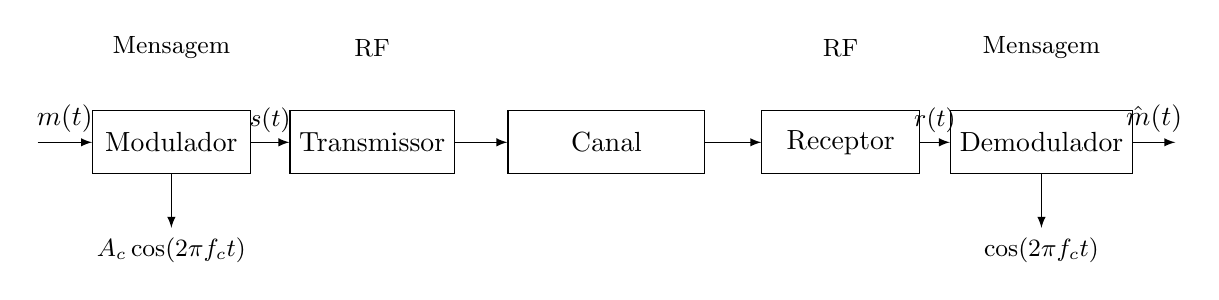
\begin{tikzpicture}[>=latex, scale=0.85]
% Transmissor
\node[draw, rectangle, minimum width=2cm, minimum height=0.8cm] (mod) at (0,0) {Modulador};
\node[draw, rectangle, minimum width=2cm, minimum height=0.8cm] (tx) at (3,0) {Transmissor};

% Canal
\node[draw, rectangle, minimum width=2.5cm, minimum height=0.8cm] (canal) at (6.5,0) {Canal};

% Receptor
\node[draw, rectangle, minimum width=2cm, minimum height=0.8cm] (rx) at (10,0) {Receptor};
\node[draw, rectangle, minimum width=2cm, minimum height=0.8cm] (demod) at (13,0) {Demodulador};

% Conexões
\draw[->] (-2,0) -- node[above] {$m(t)$} (mod.west);
\draw[->] (mod.east) -- node[above, font=\small] {$s(t)$} (tx.west);
\draw[->] (tx.east) -- (canal.west);
\draw[->] (canal.east) -- (rx.west);
\draw[->] (rx.east) -- node[above, font=\small] {$r(t)$} (demod.west);
\draw[->] (demod.east) -- node[above] {$\hat{m}(t)$} (15,0);

% Portadora
\draw[->] (mod.south) -- ++(0,-0.8) node[below, font=\small] {$A_c\cos(2\pi f_c t)$};
\draw[->] (demod.south) -- ++(0,-0.8) node[below, font=\small] {$\cos(2\pi f_c t)$};

% Labels
\node[above of=mod, node distance=1.2cm, font=\small] {Mensagem};
\node[above of=tx, node distance=1.2cm, font=\small] {RF};
\node[above of=rx, node distance=1.2cm, font=\small] {RF};
\node[above of=demod, node distance=1.2cm, font=\small] {Mensagem};
\end{tikzpicture}
\end{center}

\textbf{Componentes principais:}
\begin{itemize}
\item \textbf{Modulador:} Combina mensagem $m(t)$ com portadora
\item \textbf{Canal:} Meio de transmissão (ar, cabo, fibra)
\item \textbf{Demodulador:} Recupera $m(t)$ do sinal modulado
\end{itemize}

\end{frame}

% ============================================

\subsection{AM DSB-SC}

\begin{frame}{AM DSB-SC: Double Sideband Suppressed Carrier}

\begin{block}{Definição}
\textbf{Modulação DSB-SC:}
\[
s(t) = A_c m(t) \cos(2\pi f_c t)
\]
onde:
\begin{itemize}
\item $m(t)$: sinal modulante (mensagem) com largura de banda $W$
\item $A_c$: amplitude da portadora
\item $f_c$: frequência da portadora ($f_c \gg W$)
\end{itemize}
\end{block}

\textbf{Características:}
\begin{itemize}
\item Amplitude varia linearmente com $m(t)$
\item Portadora suprimida (não transmitida)
\item Simples de gerar: multiplicador
\item Requer detecção coerente para demodulação
\end{itemize}

\end{frame}

% ============================================

\begin{frame}{Análise Espectral do DSB-SC}

\textbf{Transformada de Fourier de} $s(t) = A_c m(t) \cos(2\pi f_c t)$:

Usando $\cos(2\pi f_c t) = \frac{e^{j2\pi f_c t} + e^{-j2\pi f_c t}}{2}$:

\[
s(t) = A_c m(t) \frac{e^{j2\pi f_c t} + e^{-j2\pi f_c t}}{2}
\]

Pela propriedade de deslocamento em frequência:
\[
m(t)e^{j2\pi f_c t} \xleftrightarrow{\mathcal{F}} M(f - f_c)
\]

Portanto:
\[
S(f) = \frac{A_c}{2}[M(f - f_c) + M(f + f_c)]
\]

\textbf{Interpretação:}
\begin{itemize}
\item Espectro de $m(t)$ deslocado para $\pm f_c$
\item \textbf{Banda Lateral Superior (USB):} $f_c$ a $f_c + W$
\item \textbf{Banda Lateral Inferior (LSB):} $f_c - W$ a $f_c$
\end{itemize}

\end{frame}

% ============================================

\begin{frame}{Largura de Banda do DSB-SC}

\[
\boxed{S(f) = \frac{A_c}{2}[M(f - f_c) + M(f + f_c)]}
\]

\textbf{Análise da largura de banda:}

\begin{itemize}
\item Mensagem $m(t)$ tem largura de banda $W$ (de $-W$ a $W$)
\item Após modulação:
  \begin{itemize}
  \item USB ocupa: $f_c$ a $f_c + W$
  \item LSB ocupa: $f_c - W$ a $f_c$
  \end{itemize}
\item Largura de banda total do sinal modulado:
\end{itemize}

\[
\boxed{B_{\DSB} = 2W}
\]

\textbf{Observações:}
\begin{itemize}
\item Ambas bandas laterais carregam a mesma informação
\item Redundância espectral
\item Oportunidade para economia de banda $\rightarrow$ SSB
\end{itemize}

\end{frame}

% ============================================

\begin{frame}{Potência do DSB-SC}

\textbf{Potência transmitida:}

\[
P_s = \frac{1}{T} \int_0^T |s(t)|^2 dt = \frac{1}{T} \int_0^T A_c^2 m^2(t) \cos^2(2\pi f_c t) dt
\]

Usando $\langle \cos^2(2\pi f_c t) \rangle = 1/2$:

\[
P_s = \frac{A_c^2}{2} \langle m^2(t) \rangle = \frac{A_c^2}{2} P_m
\]

onde $P_m$ é a potência média de $m(t)$.

\begin{block}{Potência do DSB-SC}
\[
\boxed{P_s = \frac{A_c^2 P_m}{2}}
\]
\end{block}

\textbf{Observação:}
\begin{itemize}
\item Toda potência está nas bandas laterais
\item Nenhuma potência na portadora (suprimida)
\item Eficiência energética superior ao AM convencional
\end{itemize}

\end{frame}

% ============================================

\begin{frame}{Exemplo 1: DSB-SC com Tom Único}

\textbf{Sinal modulante:} $m(t) = \cos(2\pi f_m t)$

\textbf{Sinal DSB-SC:}
\[
s(t) = A_c \cos(2\pi f_m t) \cos(2\pi f_c t)
\]

Usando identidade trigonométrica:
\[
\cos A \cos B = \frac{1}{2}[\cos(A-B) + \cos(A+B)]
\]

\[
s(t) = \frac{A_c}{2}[\cos(2\pi(f_c - f_m)t) + \cos(2\pi(f_c + f_m)t)]
\]

\textbf{Componentes espectrais:}
\begin{itemize}
\item LSB em $f_c - f_m$: amplitude $A_c/2$
\item USB em $f_c + f_m$: amplitude $A_c/2$
\item \textbf{Não há componente em $f_c$!}
\end{itemize}

\textbf{Potência:}
\[
P_s = 2 \times \frac{(A_c/2)^2}{2} = \frac{A_c^2}{4}
\]

\end{frame}

% ============================================

\begin{frame}{Demodulação Coerente do DSB-SC}

\textbf{Detector de Produto (Síncrono):}

\begin{center}
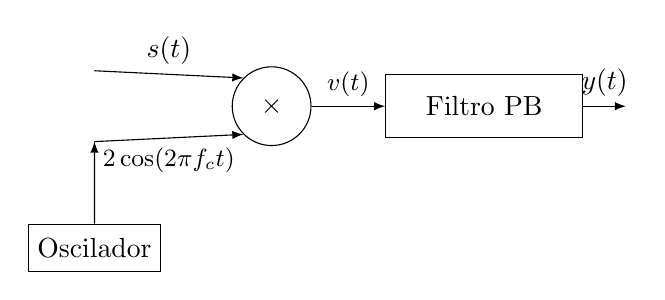
\begin{tikzpicture}[>=latex, scale=0.9]
% Multiplicador
\node[draw, circle, minimum size=1cm] (mult) at (0,0) {$\times$};
% Filtro passa-baixas
\node[draw, rectangle, minimum width=2.5cm, minimum height=0.8cm] (lpf) at (3,0) {Filtro PB};

% Entradas
\draw[->] (-2.5,0.5) -- node[above] {$s(t)$} (mult.north west);
\draw[->] (-2.5,-0.5) -- node[below, font=\small] {$2\cos(2\pi f_c t)$} (mult.south west);

% Saídas
\draw[->] (mult.east) -- node[above, font=\small] {$v(t)$} (lpf.west);
\draw[->] (lpf.east) -- node[above] {$y(t)$} (5,0);

% Oscilador local
\node[draw, rectangle, minimum width=1.5cm, minimum height=0.6cm] (osc) at (-2.5,-2) {Oscilador};
\draw[->] (osc.north) -- (-2.5,-0.5);
\end{tikzpicture}
\end{center}

\textbf{Análise matemática:}

Sinal recebido: $r(t) = A_c m(t) \cos(2\pi f_c t)$

Após multiplicação com $2\cos(2\pi f_c t)$:
\[
v(t) = 2A_c m(t) \cos^2(2\pi f_c t) = A_c m(t) [1 + \cos(4\pi f_c t)]
\]

\[
= A_c m(t) + A_c m(t) \cos(4\pi f_c t)
\]

Após filtro passa-baixas (remove $2f_c$):
\[
\boxed{y(t) = A_c m(t)}
\]

\textbf{Recuperação perfeita com ganho $A_c$!}

\end{frame}

% ============================================

\begin{frame}{Efeito de Erro de Fase na Demodulação}

\textbf{Oscilador local com erro de fase:} $2\cos(2\pi f_c t + \theta)$

Após multiplicação:
\[
v(t) = 2A_c m(t) \cos(2\pi f_c t) \cos(2\pi f_c t + \theta)
\]

Usando $\cos A \cos B = \frac{1}{2}[\cos(A-B) + \cos(A+B)]$:

\[
v(t) = A_c m(t) [\cos\theta + \cos(4\pi f_c t + \theta)]
\]

Após filtro passa-baixas:
\[
\boxed{y(t) = A_c m(t) \cos\theta}
\]

\textbf{Observações:}
\begin{itemize}
\item Atenuação por fator $\cos\theta$
\item Para $\theta = 90^{\circ}$: $y(t) = 0$ (perda total!)
\item Para $\theta pequeno$: $\cos\theta \approx 1$ (pouca degradação)
\item \textbf{Sincronização precisa é crítica!}
\end{itemize}

\end{frame}

% ============================================

\subsection{AM Convencional}

\begin{frame}{AM Convencional (DSB-LC)}

\textbf{Motivação:} DSB-SC requer sincronização perfeita. Podemos simplificar o receptor?

\begin{block}{Definição: AM Convencional}
\[
s(t) = A_c[1 + k_a m(t)] \cos(2\pi f_c t)
\]
onde:
\begin{itemize}
\item $k_a$: sensibilidade ou constante de modulação
\item $1 + k_a m(t)$: envelope do sinal
\item Condição: $|k_a m(t)| \leq 1$ (evitar supermodulação)
\end{itemize}
\end{block}

\textbf{Diferença fundamental:}
\[
s(t) = \underbrace{A_c \cos(2\pi f_c t)}_{\text{portadora}} + \underbrace{A_c k_a m(t) \cos(2\pi f_c t)}_{\text{DSB-SC}}
\]

Portadora transmitida + bandas laterais

\end{frame}

% ============================================

\begin{frame}{Índice de Modulação}

\textbf{Normalização:} Assumir $m(t)$ normalizado tal que $\max|m(t)| = 1$

\textbf{Índice de modulação:}
\[
\mu = k_a \max|m(t)| = k_a
\]

Para $0 \leq \mu \leq 1$:

\[
\boxed{s(t) = A_c[1 + \mu m_n(t)] \cos(2\pi f_c t)}
\]

onde $m_n(t)$ é $m(t)$ normalizado ($\max|m_n(t)| = 1$).

\vspace{0.3cm}

\textbf{Envelope:}
\[
A(t) = A_c[1 + \mu m_n(t)]
\]

\begin{itemize}
\item $\mu = 0$: portadora não modulada
\item $\mu = 1$: modulação 100\% (envelope vai a zero)
\item $\mu > 1$: \textbf{supermodulação} (distorção!)
\end{itemize}

\end{frame}

% ============================================

\begin{frame}{Supermodulação}

\textbf{Condição de supermodulação:} $\mu > 1$ ou $|k_a m(t)| > 1$

\textbf{Problema:}
\[
1 + k_a m(t) < 0 \quad \text{para alguns valores de } t
\]

Envelope torna-se negativo $\rightarrow$ inversão de fase $\rightarrow$ distorção

\vspace{0.5cm}

\textbf{Consequências:}
\begin{itemize}
\item Detector de envelope produz saída distorcida
\item Espectro contém componentes espúrias
\item Ineficiência de potência
\item \textbf{Deve ser evitada!}
\end{itemize}

\vspace{0.3cm}

\textbf{Solução:} Controle automático de ganho (AGC) no transmissor

\textbf{Veja figura:} Comparação de envelopes para $\mu = 0.5$, $1.0$ e $1.5$

\end{frame}

% ============================================

\begin{frame}{Espectro do AM Convencional}

\[
s(t) = A_c \cos(2\pi f_c t) + A_c k_a m(t) \cos(2\pi f_c t)
\]

\textbf{Transformada de Fourier:}
\[
S(f) = \frac{A_c}{2}[\delta(f - f_c) + \delta(f + f_c)] + \frac{A_c k_a}{2}[M(f - f_c) + M(f + f_c)]
\]

\textbf{Componentes:}
\begin{itemize}
\item \textbf{Portadora:} impulsos em $\pm f_c$ com amplitude $A_c/2$
\item \textbf{Bandas laterais:} versões deslocadas de $M(f)$
  \begin{itemize}
  \item USB: $f_c$ a $f_c + W$
  \item LSB: $f_c - W$ a $f_c$
  \end{itemize}
\end{itemize}

\textbf{Largura de banda:}
\[
B_{\AM} = 2W \quad \text{(mesma que DSB-SC)}
\]

\textbf{Diferença visual:} Presença de linhas espectrais em $\pm f_c$

\end{frame}

% ============================================

\begin{frame}{Potência do AM Convencional}

\[
s(t) = A_c[1 + k_a m(t)] \cos(2\pi f_c t)
\]

\textbf{Potência total:}
\[
P_s = \left\langle A_c^2[1 + k_a m(t)]^2 \cos^2(2\pi f_c t) \right\rangle
\]

\[
= \frac{A_c^2}{2} \left\langle [1 + k_a m(t)]^2 \right\rangle
\]

\[
= \frac{A_c^2}{2} \left[1 + 2k_a\langle m(t)\rangle + k_a^2\langle m^2(t)\rangle\right]
\]

Se $\langle m(t)\rangle = 0$ (sem componente DC):

\[
P_s = \frac{A_c^2}{2}[1 + k_a^2 P_m]
\]

\textbf{Decomposição:}
\begin{itemize}
\item Potência na portadora: $P_c = \frac{A_c^2}{2}$
\item Potência nas bandas laterais: $P_{sb} = \frac{A_c^2 k_a^2 P_m}{2}$
\end{itemize}

\end{frame}

% ============================================

\begin{frame}{Eficiência de Potência do AM}

\textbf{Eficiência:} Fração da potência total que carrega informação

\[
\eta = \frac{P_{sb}}{P_s} = \frac{P_{sb}}{P_c + P_{sb}}
\]

\[
= \frac{\frac{A_c^2 k_a^2 P_m}{2}}{\frac{A_c^2}{2} + \frac{A_c^2 k_a^2 P_m}{2}} = \frac{k_a^2 P_m}{1 + k_a^2 P_m}
\]

\textbf{Para tom único} $m(t) = \cos(2\pi f_m t)$: $P_m = 1/2$

\[
\eta = \frac{\mu^2/2}{1 + \mu^2/2} = \frac{\mu^2}{2 + \mu^2}
\]

\textbf{Eficiências típicas:}
\begin{itemize}
\item $\mu = 0.5$: $\eta = 11\%$
\item $\mu = 1.0$: $\eta = 33\%$ (máximo!)
\item $\mu = 0.3$: $\eta = 4.3\%$
\end{itemize}

\textbf{Conclusão:} AM convencional é \textbf{muito ineficiente} em potência!

\end{frame}

% ============================================

\begin{frame}{Exemplo 2: AM Convencional com Tom Único}

\textbf{Dado:} $m(t) = \cos(2\pi f_m t)$, $\mu = 0.8$, $A_c = 100$ V

\textbf{Sinal AM:}
\[
s(t) = 100[1 + 0.8\cos(2\pi f_m t)] \cos(2\pi f_c t)
\]

\textbf{Espectro:}
\begin{itemize}
\item Portadora em $f_c$: amplitude $50$ V
\item LSB em $f_c - f_m$: amplitude $40 \times 0.5 = 20$ V
\item USB em $f_c + f_m$: amplitude $20$ V
\end{itemize}

\textbf{Potências:}
\[
P_c = \frac{100^2}{2} = 5000 \text{ W (em 1 }\Omega\text{)}
\]
\[
P_{sb} = \frac{0.8^2}{2} \times 5000 = 1600 \text{ W}
\]
\[
P_s = 5000 + 1600 = 6600 \text{ W}
\]
\[
\eta = \frac{1600}{6600} = 24.2\%
\]

\end{frame}

% ============================================

\begin{frame}{Detector de Envelope}

\textbf{Vantagem do AM convencional:} Demodulação simples com detector de envelope

\begin{center}
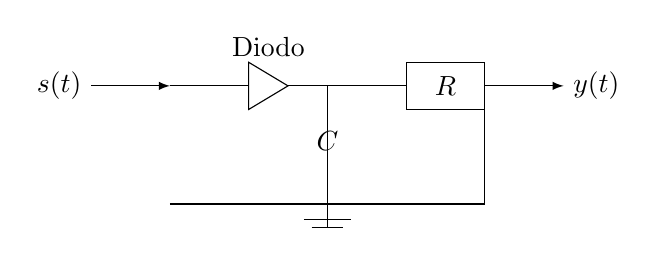
\begin{tikzpicture}[>=latex, scale=1.0]
% Diodo
\draw (0,0) -- (1,0);
\draw[fill=white] (1,-0.3) -- (1,0.3) -- (1.5,0) -- cycle;
\draw (1.5,0) -- (2,0);
% Capacitor
\draw (2,0) -- (2,-1.5);
\draw (1.7,-1.5) -- (2.3,-1.5);
\draw (1.7,-1.7) -- (2.3,-1.7);
% Resistor
\draw (2,0) -- (3,0);
\draw (3,-0.3) rectangle (4,0.3);
\node at (3.5,0) {$R$};
\draw (4,0) -- (4,-1.5);
% Terra
\draw (0,-1.5) -- (4,-1.5);
\draw (2,-1.8) -- (2,-1.5);
\draw (1.8,-1.8) -- (2.2,-1.8);
% Entrada/Saída
\draw[<-] (0,0) -- (-1,0) node[left] {$s(t)$};
\draw[->] (4,0) -- (5,0) node[right] {$y(t)$};
% Labels
\node at (2,-0.7) {$C$};
\node at (1.25,0.5) {Diodo};
\end{tikzpicture}
\end{center}

\textbf{Funcionamento:}
\begin{itemize}
\item Diodo retifica o sinal (permite apenas semi-ciclos positivos)
\item Capacitor $C$ carrega rapidamente nos picos
\item Descarrega lentamente através de $R$
\item Saída segue o envelope $A_c[1 + k_a m(t)]$
\end{itemize}

\textbf{Condição para operação correta:}
\[
\frac{1}{f_c} \ll RC \ll \frac{1}{W}
\]

\textbf{Muito mais simples que detecção coerente!} (Razão do sucesso do AM broadcast)

\end{frame}

% ============================================

\subsection{AM SSB}

\begin{frame}{AM SSB: Single Sideband}

\textbf{Observação fundamental:}

No DSB-SC, ambas bandas laterais (USB e LSB) carregam a mesma informação.

\vspace{0.3cm}

\textbf{Ideia do SSB:}

Transmitir apenas uma banda lateral $\rightarrow$ economiza largura de banda!

\vspace{0.5cm}

\textbf{Vantagens do SSB:}
\begin{itemize}
\item Largura de banda: $B_{\SSB} = W$ (metade do DSB!)
\item Potência concentrada em uma banda
\item Menos interferência
\item Melhor para canais seletivos em frequência
\end{itemize}

\textbf{Desvantagens:}
\begin{itemize}
\item Geração mais complexa
\item Demodulação coerente necessária
\item Sensível a erro de frequência
\end{itemize}

\end{frame}

% ============================================

\begin{frame}{Representação Matemática do SSB}

\textbf{SSB pode ser gerado de duas formas:}

1. Filtragem de DSB-SC
2. Método de Hilbert (phasing)

\vspace{0.5cm}

\textbf{Representação usando Transformada de Hilbert:}

\begin{block}{SSB-USB (Upper Sideband)}
\[
s_{\USB}(t) = \frac{A_c}{2}[m(t)\cos(2\pi f_c t) - \hilbert{m}(t)\sin(2\pi f_c t)]
\]
\end{block}

\begin{block}{SSB-LSB (Lower Sideband)}
\[
s_{\LSB}(t) = \frac{A_c}{2}[m(t)\cos(2\pi f_c t) + \hilbert{m}(t)\sin(2\pi f_c t)]
\]
\end{block}

onde $\hilbert{m}(t)$ é a \textbf{transformada de Hilbert} de $m(t)$.

\end{frame}

% ============================================

\begin{frame}{Transformada de Hilbert}

\begin{block}{Definição no Tempo}
\[
\hilbert{m}(t) = m(t) * \frac{1}{\pi t} = \frac{1}{\pi} \int_{-\infty}^{\infty} \frac{m(\tau)}{t - \tau} d\tau
\]
\end{block}

\begin{block}{Definição na Frequência}
\[
\hat{M}(f) = -j\sgn(f) M(f) = \begin{cases}
-jM(f) & f > 0 \\
+jM(f) & f < 0
\end{cases}
\]
\end{block}

\textbf{Interpretação:}
\begin{itemize}
\item Defasador de $-90^{\circ}$ para todas as frequências
\item Para $f > 0$: fase reduzida em $90^{\circ}$
\item Para $f < 0$: fase aumentada em $90^{\circ}$
\end{itemize}

\textbf{Exemplos:}
\begin{itemize}
\item $\hilbert{\cos(2\pi ft)} = \sin(2\pi ft)$
\item $\hilbert{\sin(2\pi ft)} = -\cos(2\pi ft)$
\end{itemize}

\end{frame}

% ============================================

\begin{frame}{Derivação do SSB-USB}

\textbf{Partindo do DSB-SC:} $s_{\DSB}(t) = A_c m(t) \cos(2\pi f_c t)$

Espectro: $S_{\DSB}(f) = \frac{A_c}{2}[M(f - f_c) + M(f + f_c)]$

\vspace{0.3cm}

\textbf{Para obter USB:} Aplicar filtro passa-altas ideal centrado em $f_c$

\[
H_{\USB}(f) = \begin{cases}
1 & f > f_c \\
0 & f < f_c
\end{cases}
\]

No tempo (método de Hilbert):

$m(t)\cos(2\pi f_c t)$ contribui para USB e LSB

$\hilbert{m}(t)\sin(2\pi f_c t)$ contribui para USB e LSB com fases opostas

\vspace{0.3cm}

\textbf{Combinação que cancela LSB:}
\[
s_{\USB}(t) = \frac{A_c}{2}[m(t)\cos(2\pi f_c t) - \hilbert{m}(t)\sin(2\pi f_c t)]
\]

LSB se cancela, USB permanece!

\end{frame}

% ============================================

\begin{frame}{Espectro do SSB}

\textbf{SSB-USB:}
\[
S_{\USB}(f) = \begin{cases}
\frac{A_c}{2}M(f - f_c) & f > 0 \\
\frac{A_c}{2}M(f + f_c) & f < 0
\end{cases}
\]

Apenas banda superior em torno de $f_c$!

\vspace{0.5cm}

\textbf{Largura de banda:}
\[
\boxed{B_{\SSB} = W}
\]

\textbf{Economia de 50\% comparado a DSB!}

\vspace{0.5cm}

\textbf{Potência:}
\[
P_{\SSB} = \frac{A_c^2 P_m}{4}
\]

Metade da potência do DSB-SC (uma banda lateral em vez de duas).

\end{frame}

% ============================================

\begin{frame}{Geração de SSB: Método do Filtro}

\begin{center}
\begin{tikzpicture}[>=latex, scale=0.85]
% Multiplicador
\node[draw, circle, minimum size=0.8cm] (mult) at (0,0) {$\times$};
% Filtro
\node[draw, rectangle, minimum width=2.2cm, minimum height=0.7cm] (filt) at (3,0) {Filtro SSB};
% Amplificador
\node[draw, rectangle, minimum width=1.5cm, minimum height=0.7cm] (amp) at (6,0) {Amp.};

% Conexões
\draw[->] (-2,0.4) -- node[above, font=\small] {$m(t)$} (mult.north west);
\draw[->] (-2,-0.4) -- node[below, font=\small] {$A_c\cos(2\pi f_c t)$} (mult.south west);
\draw[->] (mult.east) -- node[above, font=\small] {DSB-SC} (filt.west);
\draw[->] (filt.east) -- (amp.west);
\draw[->] (amp.east) -- node[above, font=\small] {$s_{\SSB}(t)$} (7.5,0);

% Resposta do filtro
\node[below of=filt, node distance=1.8cm, font=\footnotesize] (resp) {
\begin{tikzpicture}[scale=0.4]
\draw[->] (-2,0) -- (2,0) node[right] {$f$};
\draw[->] (0,-0.3) -- (0,1.5) node[above] {$|H|$};
\draw[thick, blue] (-2,0) -- (-0.3,0) -- (-0.1,1.2) -- (2,1.2);
\node[below] at (-0.2,-0.3) {$f_c$};
\end{tikzpicture}
};
\end{tikzpicture}
\end{center}

\textbf{Processo:}
\begin{enumerate}
\item Gerar DSB-SC: $A_c m(t)\cos(2\pi f_c t)$
\item Filtrar com passa-faixas centrado em $f_c$
   \begin{itemize}
   \item USB: passa alta de $f_c$
   \item LSB: passa baixa de $f_c$
   \end{itemize}
\item Amplificar
\end{enumerate}

\textbf{Desafio:} Filtro deve ter transição abrupta em $f_c$ (difícil para sinais com componentes de baixa frequência)

\end{frame}

% ============================================

\begin{frame}{Geração de SSB: Método de Hilbert}

\begin{center}
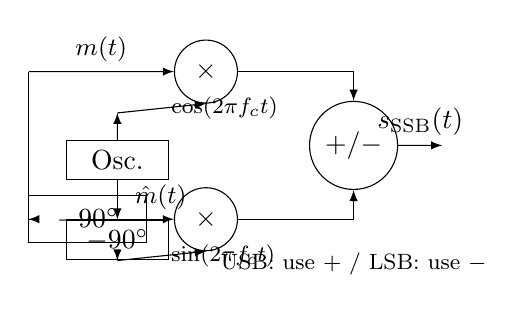
\begin{tikzpicture}[>=latex, scale=0.75]
% Branch superior
\node[draw, circle, minimum size=0.8cm] (mult1) at (2,1.5) {$\times$};
\draw[->] (-1,1.5) -- node[above, font=\small] {$m(t)$} (mult1.west);
\draw[->] (0.5,0.8) -- node[right, font=\footnotesize] {$\cos(2\pi f_c t)$} (mult1.south);

% Branch inferior
\node[draw, rectangle, minimum width=1.5cm, minimum height=0.6cm] (hilb) at (0,-1) {$-90^{\circ}$};
\node[draw, circle, minimum size=0.8cm] (mult2) at (2,-1) {$\times$};
\draw[->] (-1,1.5) |- (hilb.west);
\draw[->] (hilb.east) -- node[above, font=\small] {$\hilbert{m}(t)$} (mult2.west);
\draw[->] (0.5,-1.7) -- node[right, font=\footnotesize] {$\sin(2\pi f_c t)$} (mult2.south);

% Somador
\node[draw, circle, minimum size=0.8cm] (sum) at (4.5,0.25) {$+/-$};
\draw[->] (mult1.east) -| (sum.north);
\draw[->] (mult2.east) -| (sum.south);
\draw[->] (sum.east) -- node[above] {$s_{\SSB}(t)$} (6,0.25);

% Oscilador em fase
\node[draw, rectangle, minimum width=1.3cm, minimum height=0.5cm] (osc) at (0.5,0) {Osc.};
\draw[->] (osc.north) -- (0.5,0.8);
\node[draw, rectangle, minimum width=1.3cm, minimum height=0.5cm] (def) at (0.5,-1.35) {$-90^{\circ}$};
\draw[->] (osc.south) -- (def.north);
\draw[->] (def.south) -- (0.5,-1.7);

% Labels
\node[below of=sum, node distance=1.5cm, font=\footnotesize] {USB: use $+$ / LSB: use $-$};
\end{tikzpicture}
\end{center}

\textbf{Características:}
\begin{itemize}
\item Não requer filtros seletivos
\item Defasador de $-90^{\circ}$ (implementado com all-pass networks)
\item Dois osciladores em quadratura (defasados $90^{\circ}$)
\item Escolha do sinal no somador determina USB ou LSB
\end{itemize}

\textbf{Desafio:} Casamento preciso de amplitude e fase nos dois ramos

\end{frame}

% ============================================

\begin{frame}{Demodulação do SSB}

\textbf{SSB requer detecção coerente:}

\begin{center}
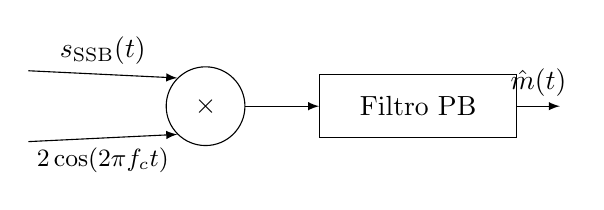
\begin{tikzpicture}[>=latex, scale=0.9]
\node[draw, circle, minimum size=1cm] (mult) at (0,0) {$\times$};
\node[draw, rectangle, minimum width=2.5cm, minimum height=0.8cm] (lpf) at (3,0) {Filtro PB};
\draw[->] (-2.5,0.5) -- node[above] {$s_{\SSB}(t)$} (mult.north west);
\draw[->] (-2.5,-0.5) -- node[below, font=\small] {$2\cos(2\pi f_c t)$} (mult.south west);
\draw[->] (mult.east) -- (lpf.west);
\draw[->] (lpf.east) -- node[above] {$\hat{m}(t)$} (5,0);
\end{tikzpicture}
\end{center}

\textbf{Sensibilidade a erro de frequência:}

Se oscilador local tem erro $\Delta f$:
\[
\hat{m}(t) = m(t) \cos(2\pi\Delta f \cdot t)
\]

Sinal recuperado tem modulação residual em $\Delta f$!

\vspace{0.3cm}

\textbf{Para voz:} $\Delta f < 20$ Hz é aceitável

\textbf{Para música:} $\Delta f < 2$ Hz necessário

\textbf{Solução:} Transmitir piloto de baixa potência para sincronização

\end{frame}

% ============================================

\begin{frame}{Exemplo 3: Comparação DSB vs SSB}

\textbf{Sinal modulante:} $m(t)$ com largura de banda $W = 5$ kHz

\textbf{Frequência da portadora:} $f_c = 1$ MHz

\vspace{0.5cm}

\textbf{Comparação:}

\begin{center}
\begin{tabular}{|l|c|c|}
\hline
\textbf{Característica} & \textbf{DSB-SC} & \textbf{SSB} \\
\hline
Largura de banda & $2W = 10$ kHz & $W = 5$ kHz \\
\hline
Potência (relativa) & $1.0$ & $0.5$ \\
\hline
Geração & Simples & Complexa \\
\hline
Demodulação & Coerente & Coerente \\
\hline
Sensibilidade $\Delta f$ & Baixa & Alta \\
\hline
Aplicações & Estéreo FM & Rádio amador \\
& & Comunicação longa distância \\
\hline
\end{tabular}
\end{center}

\textbf{Trade-off:} Economia de banda vs. complexidade

\end{frame}

% ============================================

\subsection{AM VSB}

\begin{frame}{AM VSB: Vestigial Sideband}

\textbf{Problema com SSB:}

Filtragem abrupta em $f_c$ é difícil, especialmente para sinais com componentes DC ou de muito baixa frequência (ex: vídeo).

\vspace{0.3cm}

\textbf{Solução: VSB}

Transmitir uma banda lateral completa + "vestígio" da outra.

\begin{block}{Definição}
VSB é um compromisso entre DSB e SSB:
\begin{itemize}
\item Largura de banda: $W < B_{\VSB} < 2W$
\item Transmite USB completa + parte da LSB (ou vice-versa)
\item Filtro com roll-off gradual em $f_c$
\end{itemize}
\end{block}

\textbf{Aplicação principal:} TV analógica (NTSC, PAL)

Vídeo tem componentes de 0 Hz a vários MHz $\rightarrow$ SSB impraticável

\end{frame}

% ============================================

\begin{frame}{Filtro VSB}

\textbf{Característica do filtro VSB:}

\begin{center}
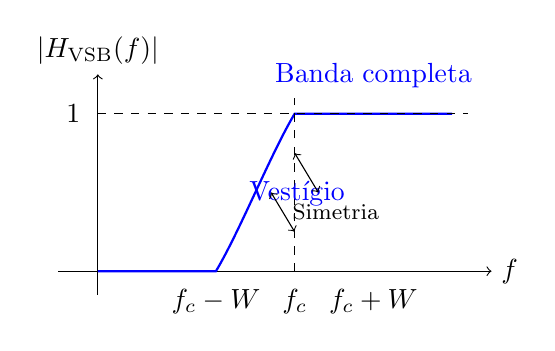
\begin{tikzpicture}[scale=1.0]
\draw[->] (-0.5,0) -- (5,0) node[right] {$f$};
\draw[->] (0,-0.3) -- (0,2.5) node[above] {$|H_{\VSB}(f)|$};

% Filtro VSB
\draw[thick, blue] (0,0) -- (1.5,0) 
    .. controls (1.8,0.5) and (2.2,1.5) .. 
    (2.5,2) -- (4.5,2);

% Linhas de referência
\draw[dashed] (2.5,0) -- (2.5,2.2);
\draw[dashed] (0,2) -- (4.7,2);

% Labels
\node[below] at (2.5,-0.1) {$f_c$};
\node[left] at (-0.1,2) {$1$};
\node[below] at (1.5,-0.1) {$f_c-W$};
\node[below] at (3.5,-0.1) {$f_c+W$};
\node[above right, blue] at (1.8,0.7) {Vestígio};
\node[above, blue] at (3.5,2.2) {Banda completa};

% Simetria vestigial
\draw[<->] (2.5,0.5) -- (2.2,1) node[midway, right, font=\footnotesize] {Simetria};
\draw[<->] (2.5,1.5) -- (2.8,1);
\end{tikzpicture}
\end{center}

\textbf{Condição de simetria vestigial:}
\[
H_{\VSB}(f_c + f) + H_{\VSB}(f_c - f) = \text{constante}
\]

Garante recuperação sem distorção na demodulação coerente.

\end{frame}

% ============================================

\begin{frame}{Análise Matemática do VSB}

\textbf{Sinal VSB:}
\[
s_{\VSB}(t) = [A_c m(t) \cos(2\pi f_c t)] * h_{\VSB}(t)
\]

\textbf{No domínio da frequência:}
\[
S_{\VSB}(f) = \frac{A_c}{2}[M(f - f_c) + M(f + f_c)] H_{\VSB}(f)
\]

\textbf{Demodulação coerente com} $2\cos(2\pi f_c t)$:

Produto resulta em:
\[
v(t) = s_{\VSB}(t) \cdot 2\cos(2\pi f_c t)
\]

Após passa-baixas, se $H_{\VSB}$ satisfaz condição de simetria:
\[
\boxed{y(t) = A_c m(t)}
\]

\textbf{Recuperação perfeita!}

\end{frame}

% ============================================

\begin{frame}{VSB na TV Analógica}

\textbf{Sistema NTSC (EUA):}

\begin{itemize}
\item Sinal de vídeo: 0 a 4.2 MHz
\item Frequência de portadora visual: $f_v$
\item Largura do canal: 6 MHz total
\end{itemize}

\textbf{Alocação espectral:}
\begin{itemize}
\item Vestígio LSB: 1.25 MHz abaixo de $f_v$
\item USB completa: 4.2 MHz acima de $f_v$
\item Portadora de áudio FM: 4.5 MHz acima de $f_v$
\end{itemize}

\textbf{Economia de banda:}
\begin{itemize}
\item DSB precisaria: $2 \times 4.2 = 8.4$ MHz
\item VSB usa: $1.25 + 4.2 = 5.45$ MHz
\item Economia: $\approx 35\%$
\end{itemize}

\textbf{Trade-off perfeito:} Eficiência espectral + facilidade de implementação

\end{frame}

% ============================================

\begin{frame}{Largura de Banda do VSB}

\textbf{Largura de banda geral:}
\[
B_{\VSB} = W + f_{vest}
\]

onde $f_{vest}$ é a largura do vestígio.

\vspace{0.3cm}

\textbf{Limites:}
\begin{itemize}
\item Se $f_{vest} = W$: $B_{\VSB} = 2W$ (torna-se DSB)
\item Se $f_{vest} = 0$: $B_{\VSB} = W$ (torna-se SSB)
\end{itemize}

\textbf{Típico:} $f_{vest} = 0.2W$ a $0.3W$

\[
\boxed{W < B_{\VSB} < 2W}
\]

\textbf{Exemplo NTSC:}
\begin{itemize}
\item $W = 4.2$ MHz
\item $f_{vest} = 1.25$ MHz
\item $B_{\VSB} = 5.45$ MHz $\approx 1.3W$
\end{itemize}

\end{frame}

% ============================================

\subsection{Comparação}

\begin{frame}{Tabela Comparativa: Tipos de AM}

\begin{center}
\footnotesize
\begin{tabular}{|l|c|c|c|c|}
\hline
\textbf{Tipo} & \textbf{DSB-SC} & \textbf{AM Conv.} & \textbf{SSB} & \textbf{VSB} \\
\hline
Largura de banda & $2W$ & $2W$ & $W$ & $W<B<2W$ \\
\hline
Potência (relativa) & $1.0$ & $>3.0$ & $0.5$ & $\approx 0.7$ \\
\hline
Eficiência potência & Alta & Baixa & Máxima & Alta \\
& & $(< 33\%)$ & & \\
\hline
Geração & Simples & Simples & Complexa & Moderada \\
\hline
Demodulação & Coerente & Envelope & Coerente & Coerente \\
\hline
Complexidade RX & Média & Mínima & Alta & Média \\
\hline
Sensibilidade $\Delta f$ & Baixa & N/A & Alta & Média \\
\hline
Aplicações & - & Rádio AM & Rádio & TV \\
& & broadcast & amador & analógica \\
\hline
\end{tabular}
\end{center}

\vspace{0.3cm}

\textbf{Escolha depende de:}
\begin{itemize}
\item Largura de banda disponível
\item Potência disponível
\item Complexidade aceitável no TX e RX
\item Custo
\end{itemize}

\end{frame}

% ============================================

\begin{frame}{Comparação Espectral Visual}

\textbf{Para mesmo sinal modulante} $m(t)$ com banda $W$:

\begin{center}
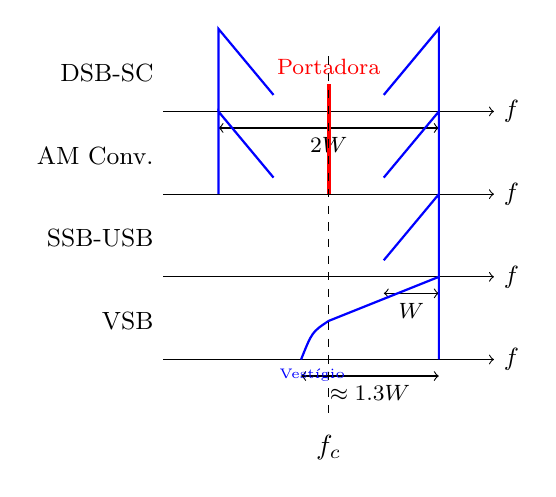
\begin{tikzpicture}[scale=0.7]
% DSB-SC
\begin{scope}[yshift=3cm]
\draw[->] (-3,0) -- (3,0) node[right, font=\small] {$f$};
\draw[thick, blue] (-2,0) -- (-2,1.5) -- (-1,0.3);
\draw[thick, blue] (1,0.3) -- (2,1.5) -- (2,0);
\node[left, font=\small] at (-3,0.7) {DSB-SC};
\draw[<->] (-2,-0.3) -- (2,-0.3) node[midway, below, font=\footnotesize] {$2W$};
\end{scope}

% AM Convencional
\begin{scope}[yshift=1.5cm]
\draw[->] (-3,0) -- (3,0) node[right, font=\small] {$f$};
\draw[thick, blue] (-2,0) -- (-2,1.5) -- (-1,0.3);
\draw[thick, blue] (1,0.3) -- (2,1.5) -- (2,0);
\draw[thick, red, line width=1.5pt] (0,0) -- (0,2);
\node[left, font=\small] at (-3,0.7) {AM Conv.};
\node[above, red, font=\footnotesize] at (0,2) {Portadora};
\end{scope}

% SSB
\begin{scope}[yshift=0cm]
\draw[->] (-3,0) -- (3,0) node[right, font=\small] {$f$};
\draw[thick, blue] (1,0.3) -- (2,1.5) -- (2,0);
\node[left, font=\small] at (-3,0.7) {SSB-USB};
\draw[<->] (1,-0.3) -- (2,-0.3) node[midway, below, font=\footnotesize] {$W$};
\end{scope}

% VSB
\begin{scope}[yshift=-1.5cm]
\draw[->] (-3,0) -- (3,0) node[right, font=\small] {$f$};
\draw[thick, blue] (-0.5,0) .. controls (-0.3,0.5) .. (0,0.7) 
                   -- (2,1.5) -- (2,0);
\node[left, font=\small] at (-3,0.7) {VSB};
\draw[<->] (-0.5,-0.3) -- (2,-0.3) node[midway, below, font=\footnotesize] {$\approx 1.3W$};
\node[below, blue, font=\tiny] at (-0.3,0) {Vestígio};
\end{scope}

% fc marca
\draw[dashed] (0,4) -- (0,-2.5);
\node[below] at (0,-2.7) {$f_c$};
\end{tikzpicture}
\end{center}

\end{frame}

% ============================================

\begin{frame}{Aplicações Práticas das Variantes AM}

\textbf{AM Convencional (DSB-LC):}
\begin{itemize}
\item Rádio AM broadcast (535-1705 kHz)
\item Receptor muito simples e barato
\item Ainda usado em países em desenvolvimento
\end{itemize}

\textbf{SSB:}
\begin{itemize}
\item Rádio amador (HF: 3-30 MHz)
\item Comunicações marítimas e aeronáuticas
\item Comunicações militares de longa distância
\item Telefonia por satélite (histórico)
\end{itemize}

\textbf{VSB:}
\begin{itemize}
\item TV analógica terrestre (NTSC, PAL, SECAM)
\item Modems de alta velocidade (histórico)
\item Base para VSB digital (ATSC)
\end{itemize}

\textbf{DSB-SC:}
\begin{itemize}
\item Estéreo em FM (sinal L-R)
\item Componente de cor em TV (QAM)
\end{itemize}

\end{frame}

% ============================================

\begin{frame}{Resumo: Modulação em Amplitude}

\textbf{Conceitos fundamentais:}
\begin{itemize}
\item Modulação desloca espectro de banda base para RF
\item Facilita multiplexação, propagação e processamento
\end{itemize}

\vspace{0.3cm}

\textbf{Quatro variantes principais:}

\begin{enumerate}
\item \textbf{DSB-SC:} $s(t) = A_c m(t)\cos(2\pi f_c t)$
   \begin{itemize}
   \item Simples, mas requer detecção coerente
   \end{itemize}

\item \textbf{AM Convencional:} $s(t) = A_c[1 + k_a m(t)]\cos(2\pi f_c t)$
   \begin{itemize}
   \item Detector de envelope, mas ineficiente ($\eta \leq 33\%$)
   \end{itemize}

\item \textbf{SSB:} Usa transformada de Hilbert
   \begin{itemize}
   \item Economiza largura de banda (50\%)
   \end{itemize}

\item \textbf{VSB:} Compromisso DSB-SSB
   \begin{itemize}
   \item Ideal para sinais com componentes DC/baixa frequência
   \end{itemize}
\end{enumerate}

\textbf{Escolha baseada em:} Banda disponível, potência, complexidade, custo

\end{frame}


% ============================================
% MODULAÇÃO EM FREQUÊNCIA (FM) E FASE (PM)
% ============================================
\section{Modulação Angular: FM e PM}
% ============================================
% MODULAÇÃO ANGULAR: FM E PM
% ============================================

\subsection{Introdução}

\begin{frame}{Modulação Angular vs. Modulação em Amplitude}

\textbf{AM:} Amplitude varia, frequência e fase fixas
\[
s_{\AM}(t) = A(t) \cos(2\pi f_c t)
\]

\vspace{0.3cm}

\textbf{Modulação Angular:} Amplitude fixa, ângulo (fase ou frequência) varia
\[
s(t) = A_c \cos[\theta(t)] = A_c \cos[2\pi f_c t + \phi(t)]
\]

onde $\phi(t)$ é a fase modulada.

\vspace{0.5cm}

\textbf{Duas variantes:}

\begin{enumerate}
\item \textbf{FM (Modulação em Frequência):}
   
   Frequência instantânea varia com $m(t)$

\item \textbf{PM (Modulação em Fase):}
   
   Fase instantânea varia diretamente com $m(t)$
\end{enumerate}

\end{frame}

% ============================================

\begin{frame}{Fase e Frequência Instantâneas}

Para sinal modulado $s(t) = A_c \cos[\theta(t)]$:

\begin{block}{Definições}
\textbf{Fase instantânea:}
\[
\theta(t) = 2\pi f_c t + \phi(t)
\]

\textbf{Frequência instantânea:}
\[
f_i(t) = \frac{1}{2\pi} \frac{d\theta(t)}{dt} = f_c + \frac{1}{2\pi}\frac{d\phi(t)}{dt}
\]
\end{block}

\textbf{Interpretação:}
\begin{itemize}
\item $\theta(t)$: argumento da função cosseno
\item $f_i(t)$: taxa instantânea de oscilação
\item $f_c$: frequência da portadora (não modulada)
\item $\phi(t)$: desvio de fase causado pela modulação
\end{itemize}

\end{frame}

% ============================================

\subsection{Modulação em Frequência (FM)}

\begin{frame}{Definição de FM}

\begin{block}{Modulação em Frequência (FM)}
A frequência instantânea é proporcional à mensagem:
\[
f_i(t) = f_c + k_f m(t)
\]
onde $k_f$ é a constante de sensibilidade de frequência (Hz/V).
\end{block}

\textbf{Desvio de frequência:}
\[
\Delta f(t) = k_f m(t)
\]

\textbf{Desvio máximo:}
\[
\Delta f = k_f \max|m(t)|
\]

\vspace{0.3cm}

\textbf{Derivando} $\phi(t)$ de $f_i(t)$:

\[
\frac{d\phi(t)}{dt} = 2\pi k_f m(t) \quad \Rightarrow \quad \phi(t) = 2\pi k_f \int_{-\infty}^{t} m(\tau) d\tau
\]

\end{frame}

% ============================================

\begin{frame}{Sinal FM no Domínio do Tempo}

\begin{block}{Sinal FM}
\[
s_{\FM}(t) = A_c \cos\left[2\pi f_c t + 2\pi k_f \int_{-\infty}^{t} m(\tau) d\tau\right]
\]
\end{block}

Ou definindo o \textbf{índice de fase}:
\[
\beta(t) = 2\pi k_f \int_{-\infty}^{t} m(\tau) d\tau
\]

\[
s_{\FM}(t) = A_c \cos[2\pi f_c t + \beta(t)]
\]

\textbf{Características:}
\begin{itemize}
\item Amplitude constante: $|s_{\FM}(t)| = A_c$
\item Toda informação está na fase
\item Potência transmitida constante: $P_s = A_c^2/2$
\item \textbf{Vantagem:} Imune a variações de amplitude (ruído, desvanecimento)
\end{itemize}

\end{frame}

% ============================================

\begin{frame}{Modulação em Fase (PM)}

\begin{block}{Modulação em Fase (PM)}
A fase instantânea é diretamente proporcional à mensagem:
\[
\phi(t) = k_p m(t)
\]
onde $k_p$ é a constante de sensibilidade de fase (rad/V).
\end{block}

\textbf{Sinal PM:}
\[
s_{\PM}(t) = A_c \cos[2\pi f_c t + k_p m(t)]
\]

\textbf{Frequência instantânea:}
\[
f_i(t) = f_c + \frac{k_p}{2\pi} \frac{dm(t)}{dt}
\]

\textbf{Relação FM-PM:}
\begin{itemize}
\item \textbf{FM:} frequência $\propto m(t)$, fase $\propto \int m(t)dt$
\item \textbf{PM:} fase $\propto m(t)$, frequência $\propto dm(t)/dt$
\end{itemize}

\end{frame}

% ============================================

\begin{frame}{Relação entre FM e PM}

\textbf{FM pode ser vista como PM do integral:}

\[
\text{FM de } m(t) = \text{PM de } \int m(t)dt
\]

\textbf{PM pode ser vista como FM da derivada:}

\[
\text{PM de } m(t) = \text{FM de } \frac{dm(t)}{dt}
\]

\vspace{0.5cm}

\textbf{Conversão prática:}

\begin{center}
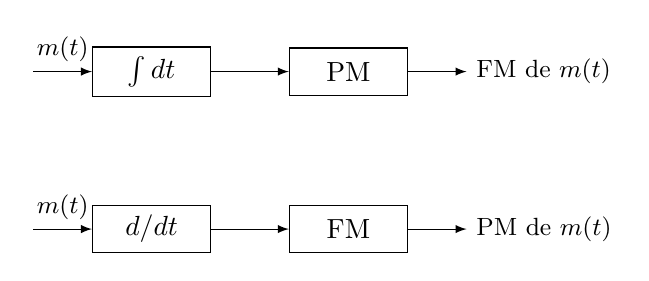
\begin{tikzpicture}[>=latex]
% FM para PM
\node[draw, rectangle, minimum width=1.5cm, minimum height=0.6cm] (int) at (0,1) {$\int dt$};
\node[draw, rectangle, minimum width=1.5cm, minimum height=0.6cm] (pm) at (2.5,1) {PM};
\draw[->] (-1.5,1) -- node[above, font=\small] {$m(t)$} (int);
\draw[->] (int) -- (pm);
\draw[->] (pm) -- (4,1) node[right, font=\small] {FM de $m(t)$};

% PM para FM
\node[draw, rectangle, minimum width=1.5cm, minimum height=0.6cm] (der) at (0,-1) {$d/dt$};
\node[draw, rectangle, minimum width=1.5cm, minimum height=0.6cm] (fm) at (2.5,-1) {FM};
\draw[->] (-1.5,-1) -- node[above, font=\small] {$m(t)$} (der);
\draw[->] (der) -- (fm);
\draw[->] (fm) -- (4,-1) node[right, font=\small] {PM de $m(t)$};
\end{tikzpicture}
\end{center}

\textbf{Na prática:} FM é mais comum (melhor desempenho em ruído)

\end{frame}

% ============================================

\subsection{Análise Espectral de FM}

\begin{frame}{FM com Tom Único: Configuração}

\textbf{Sinal modulante:} $m(t) = A_m \cos(2\pi f_m t)$

\textbf{Sinal FM:}
\[
s(t) = A_c \cos\left[2\pi f_c t + 2\pi k_f A_m \int_{-\infty}^{t} \cos(2\pi f_m \tau) d\tau\right]
\]

Integrando:
\[
\int \cos(2\pi f_m \tau) d\tau = \frac{\sin(2\pi f_m t)}{2\pi f_m}
\]

\[
s(t) = A_c \cos\left[2\pi f_c t + \frac{k_f A_m}{f_m} \sin(2\pi f_m t)\right]
\]

Definindo o \textbf{índice de modulação}:
\[
\beta = \frac{k_f A_m}{f_m} = \frac{\Delta f}{f_m}
\]

\[
\boxed{s(t) = A_c \cos[2\pi f_c t + \beta \sin(2\pi f_m t)]}
\]

\end{frame}

% ============================================

\begin{frame}{Expansão de Bessel}

\textbf{Para analisar o espectro, usamos a identidade:}

\[
\cos[\beta \sin(\omega_m t)] = \sum_{n=-\infty}^{\infty} J_n(\beta) \cos(n\omega_m t)
\]

onde $J_n(\beta)$ são \textbf{funções de Bessel de primeira espécie de ordem $n$}.

\vspace{0.3cm}

\textbf{Aplicando a} $s(t) = A_c \cos[2\pi f_c t + \beta \sin(2\pi f_m t)]$:

Usando $\cos(A + B) = \cos A \cos B - \sin A \sin B$:

\[
s(t) = A_c[\cos(2\pi f_c t)\cos(\beta \sin(2\pi f_m t)) - \sin(2\pi f_c t)\sin(\beta \sin(2\pi f_m t))]
\]

E as identidades:
\begin{align*}
\cos[\beta \sin(\omega_m t)] &= J_0(\beta) + 2\sum_{n=1}^{\infty} J_{2n}(\beta) \cos(2n\omega_m t) \\
\sin[\beta \sin(\omega_m t)] &= 2\sum_{n=0}^{\infty} J_{2n+1}(\beta) \sin[(2n+1)\omega_m t]
\end{align*}

\end{frame}

% ============================================

\begin{frame}{Espectro FM: Resultado Final}

Após manipulação algébrica:

\[
s(t) = A_c \sum_{n=-\infty}^{\infty} J_n(\beta) \cos[2\pi(f_c + nf_m)t]
\]

\textbf{Interpretação do espectro:}

\begin{itemize}
\item \textbf{Portadora} em $f_c$: amplitude $A_c J_0(\beta)$
\item \textbf{Bandas laterais} em $f_c \pm nf_m$ para $n = 1, 2, 3, ...$
\item Amplitude da n-ésima banda: $A_c J_n(\beta)$
\item \textbf{Infinitas bandas laterais teoricamente}
\item Na prática: $J_n(\beta) \approx 0$ para $n > \beta + 1$
\end{itemize}

\vspace{0.3cm}

\textbf{Diferença fundamental de AM:}
\begin{itemize}
\item AM: 2 bandas laterais (USB, LSB)
\item FM: Infinitas bandas laterais (mas só algumas significativas)
\end{itemize}

\end{frame}

% ============================================

\begin{frame}{Funções de Bessel}

\textbf{Propriedades importantes:}

\begin{itemize}
\item $J_{-n}(\beta) = (-1)^n J_n(\beta)$ (simetria)
\item $J_n(-\beta) = (-1)^n J_n(\beta)$
\item $\sum_{n=-\infty}^{\infty} J_n^2(\beta) = 1$ (conservação de potência!)
\item Para $\beta \ll 1$: $J_0(\beta) \approx 1$, $J_1(\beta) \approx \beta/2$, $J_n(\beta) \approx 0$ para $n \geq 2$
\end{itemize}

\vspace{0.3cm}

\textbf{Valores típicos:}

\begin{center}
\footnotesize
\begin{tabular}{|c|c|c|c|c|c|c|}
\hline
$\beta$ & $J_0$ & $J_1$ & $J_2$ & $J_3$ & $J_4$ & $J_5$ \\
\hline
0.5 & 0.94 & 0.24 & 0.03 & 0.00 & - & - \\
\hline
1.0 & 0.77 & 0.44 & 0.11 & 0.02 & 0.00 & - \\
\hline
2.0 & 0.22 & 0.58 & 0.35 & 0.13 & 0.03 & 0.01 \\
\hline
5.0 & -0.18 & -0.33 & 0.05 & 0.36 & 0.39 & 0.26 \\
\hline
\end{tabular}
\end{center}

\textbf{Veja figura:} Gráfico de $J_n(\beta)$ vs. $\beta$ para diferentes $n$

\end{frame}

% ============================================

\begin{frame}{Largura de Banda de FM}

\textbf{Problema:} Teoricamente, espectro FM tem largura infinita!

Na prática: Bandas com $|J_n(\beta)| < 0.01$ são desprezíveis.

\vspace{0.3cm}

\textbf{Número significativo de bandas laterais:}

Aproximadamente $n_{\max} \approx \beta + 1$

\textbf{Largura de banda aproximada:}
\[
B \approx 2n_{\max} f_m = 2(\beta + 1)f_m
\]

\begin{block}{Regra de Carson}
\[
\boxed{B_{\FM} \approx 2(\Delta f + f_m) = 2f_m(\beta + 1)}
\]
\end{block}

onde $\Delta f = k_f A_m$ é o desvio de frequência.

\textbf{Precisão:} Contém $\approx 98\%$ da potência do sinal FM.

\end{frame}

% ============================================

\begin{frame}{NBFM vs. WBFM}

\textbf{Dois regimes de operação:}

\begin{enumerate}
\item \textbf{NBFM (Narrowband FM):} $\beta \ll 1$
   \begin{itemize}
   \item $B \approx 2f_m$ (similar a AM)
   \item Poucas bandas laterais significativas
   \item Comportamento quase linear
   \end{itemize}

\item \textbf{WBFM (Wideband FM):} $\beta \gg 1$
   \begin{itemize}
   \item $B \approx 2\Delta f$ (dominado pelo desvio)
   \item Muitas bandas laterais
   \item Melhor desempenho em ruído
   \end{itemize}
\end{enumerate}

\vspace{0.3cm}

\textbf{Comparação com AM:}

\begin{itemize}
\item AM: $B = 2W$ (independente de $A_c$ ou $\mu$)
\item FM: $B = 2\Delta f(1 + 1/\beta)$ (depende de $\Delta f$!)
\item FM troca largura de banda por melhor SNR
\end{itemize}

\end{frame}

% ============================================

\begin{frame}{Exemplo 1: FM com Tom Único}

\textbf{Dados:}
\begin{itemize}
\item $m(t) = \cos(2\pi \times 5000 \cdot t)$ (5 kHz)
\item $\Delta f = 75$ kHz (desvio máximo)
\item $f_c = 100$ MHz (portadora)
\end{itemize}

\textbf{Cálculo do índice de modulação:}
\[
\beta = \frac{\Delta f}{f_m} = \frac{75 \text{ kHz}}{5 \text{ kHz}} = 15
\]

\textbf{Largura de banda (Carson):}
\[
B \approx 2(\Delta f + f_m) = 2(75 + 5) = 160 \text{ kHz}
\]

\textbf{Número de bandas significativas:}
\[
n_{\max} \approx \beta + 1 = 16
\]

$\rightarrow$ 16 pares de bandas laterais (32 componentes espectrais!)

\textbf{Classificação:} WBFM ($\beta = 15 \gg 1$)

\end{frame}

% ============================================

\begin{frame}{Exemplo 2: Rádio FM Comercial}

\textbf{Padrão FCC para FM broadcast:}

\begin{itemize}
\item Desvio máximo: $\Delta f = 75$ kHz
\item Frequência máxima de áudio: $f_m = 15$ kHz
\item Alocação de canal: 200 kHz
\end{itemize}

\textbf{Índice de modulação:}
\[
\beta = \frac{75 \text{ kHz}}{15 \text{ kHz}} = 5
\]

\textbf{Largura de banda necessária:}
\[
B = 2(\Delta f + f_m) = 2(75 + 15) = 180 \text{ kHz}
\]

\textbf{Observação:} Canal de 200 kHz acomoda 180 kHz + bandas de guarda

\vspace{0.3cm}

\textbf{Banda FM:} 88-108 MHz, espaçamento de 200 kHz

Número de canais: $(108-88)/0.2 = 100$ canais

\end{frame}

% ============================================

\subsection{Demodulação FM}

\begin{frame}{Princípios de Demodulação FM}

\textbf{Objetivo:} Recuperar $m(t)$ de $s_{\FM}(t) = A_c \cos[2\pi f_c t + 2\pi k_f \int m(\tau)d\tau]$

\vspace{0.3cm}

\textbf{Métodos principais:}

\begin{enumerate}
\item \textbf{Discriminador de frequência (slope detector)}
   \begin{itemize}
   \item Converte FM em AM, depois detecta envelope
   \end{itemize}

\item \textbf{Detector PLL (Phase-Locked Loop)}
   \begin{itemize}
   \item VCO "segue" a frequência de entrada
   \item Saída do VCO é proporcional a $m(t)$
   \end{itemize}

\item \textbf{Detector de Foster-Seeley}
   \begin{itemize}
   \item Usa transformador balanceado
   \end{itemize}

\item \textbf{Detector de razão (ratio detector)}
   \begin{itemize}
   \item Variante do Foster-Seeley
   \item Menos sensível a variações de amplitude
   \end{itemize}
\end{enumerate}

\end{frame}

% ============================================

\begin{frame}{Discriminador de Frequência}

\textbf{Princípio:} Converter variação de frequência em variação de amplitude

\begin{center}
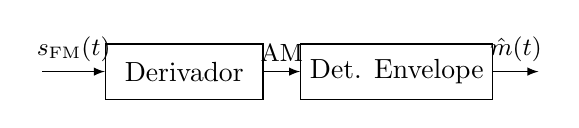
\begin{tikzpicture}[>=latex, scale=0.9]
\node[draw, rectangle, minimum width=2cm, minimum height=0.7cm] (der) at (0,0) {Derivador};
\node[draw, rectangle, minimum width=2cm, minimum height=0.7cm] (env) at (3,0) {Det. Envelope};

\draw[->] (-2,0) -- node[above, font=\small] {$s_{\FM}(t)$} (der);
\draw[->] (der) -- node[above, font=\small] {AM} (env);
\draw[->] (env) -- node[above, font=\small] {$\hat{m}(t)$} (5,0);
\end{tikzpicture}
\end{center}

\textbf{Análise matemática:}

\[
\frac{ds_{\FM}(t)}{dt} = -A_c \cdot 2\pi f_i(t) \sin[2\pi f_c t + \phi(t)]
\]

Amplitude do sinal derivado:
\[
A(t) = 2\pi A_c f_i(t) = 2\pi A_c [f_c + k_f m(t)]
\]

Após detector de envelope e filtro DC:
\[
\hat{m}(t) = K \cdot k_f m(t)
\]

\textbf{Problema:} Sensível a variações de amplitude (ruído AM)

\textbf{Solução:} Limitador de amplitude antes do discriminador

\end{frame}

% ============================================

\begin{frame}{Limitador de Amplitude}

\textbf{Propósito:} Remover variações de amplitude antes da demodulação FM

\begin{center}
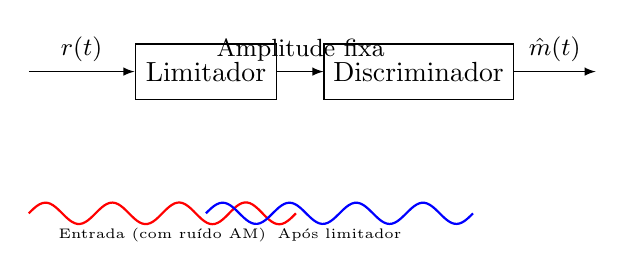
\begin{tikzpicture}[>=latex, scale=0.9]
\node[draw, rectangle, minimum width=1.8cm, minimum height=0.7cm] (lim) at (0,0) {Limitador};
\node[draw, rectangle, minimum width=2.2cm, minimum height=0.7cm] (disc) at (3,0) {Discriminador};

\draw[->] (-2.5,0) -- node[above, font=\small] {$r(t)$} (lim);
\draw[->] (lim) -- node[above, font=\small] {Amplitude fixa} (disc);
\draw[->] (disc) -- node[above, font=\small] {$\hat{m}(t)$} (5.5,0);

% Forma de onda de entrada (com variação de amplitude)
\begin{scope}[xshift=-2.5cm, yshift=-2cm, scale=0.15]
\draw[thick, red] plot[domain=0:8*pi, samples=100] (\x, {(1+0.3*sin(\x/4))*sin(\x r)});
\node[font=\tiny] at (4*pi,-2) {Entrada (com ruído AM)};
\end{scope}

% Forma de onda de saída (amplitude constante)
\begin{scope}[xshift=0cm, yshift=-2cm, scale=0.15]
\draw[thick, blue] plot[domain=0:8*pi, samples=100] (\x, {sin(\x r)});
\node[font=\tiny] at (4*pi,-2) {Após limitador};
\end{scope}
\end{tikzpicture}
\end{center}

\textbf{Implementação:}
\begin{itemize}
\item Amplificador com saturação (clipper)
\item Mantém informação de FM
\item Remove variações de amplitude
\end{itemize}

\textbf{Vantagem de FM:} Informação na frequência, não na amplitude!

\end{frame}

% ============================================

\subsection{PLL (Phase-Locked Loop)}

\begin{frame}{Conceito do PLL}

\textbf{PLL (Phase-Locked Loop):} Sistema de controle realimentado que sincroniza um oscilador local com sinal de entrada.

\begin{center}
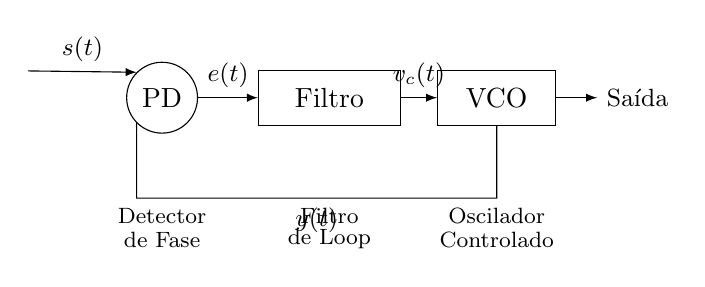
\begin{tikzpicture}[>=latex, scale=0.85]
% Detector de fase
\node[draw, circle, minimum size=0.9cm] (pd) at (0,0) {PD};
% Filtro
\node[draw, rectangle, minimum width=1.8cm, minimum height=0.7cm] (lpf) at (2.5,0) {Filtro};
% VCO
\node[draw, rectangle, minimum width=1.5cm, minimum height=0.7cm] (vco) at (5,0) {VCO};

% Conexões
\draw[->] (-2,0.4) -- node[above, font=\small] {$s(t)$} (pd.north west);
\draw[->] (pd.east) -- node[above, font=\small] {$e(t)$} (lpf.west);
\draw[->] (lpf.east) -- node[above, font=\small] {$v_c(t)$} (vco.west);
\draw[->] (vco.east) -- (6.5,0) node[right, font=\small] {Saída};

% Realimentação
\draw (vco.south) -- (5,-1.5) -| node[below, pos=0.25, font=\small] {$y(t)$} (pd.south west);

% Labels
\node[below of=pd, node distance=1.5cm, font=\footnotesize] {Detector};
\node[below of=pd, node distance=1.8cm, font=\footnotesize] {de Fase};
\node[below of=lpf, node distance=1.5cm, font=\footnotesize] {Filtro};
\node[below of=lpf, node distance=1.8cm, font=\footnotesize] {de Loop};
\node[below of=vco, node distance=1.5cm, font=\footnotesize] {Oscilador};
\node[below of=vco, node distance=1.8cm, font=\footnotesize] {Controlado};
\end{tikzpicture}
\end{center}

\textbf{Componentes:}
\begin{itemize}
\item \textbf{Detector de fase (PD):} Compara fases de entrada e VCO
\item \textbf{Filtro de loop:} Passa-baixas, define dinâmica
\item \textbf{VCO:} Frequência controlada por tensão
\end{itemize}

\end{frame}

% ============================================

\begin{frame}{Análise do PLL}

\textbf{Sinal de entrada FM:}
\[
s(t) = A_c \cos[2\pi f_c t + \phi_i(t)]
\]

\textbf{Saída do VCO:}
\[
y(t) = A_v \cos[2\pi f_c t + \phi_o(t)]
\]

\textbf{Detector de fase (multiplicador):}
\[
e(t) = K_d \sin[\phi_i(t) - \phi_o(t)] \approx K_d[\phi_i(t) - \phi_o(t)]
\]

para pequenos erros de fase.

\textbf{VCO:}
\[
\frac{d\phi_o(t)}{dt} = 2\pi K_v v_c(t)
\]

onde $K_v$ é a sensibilidade do VCO (Hz/V).

\end{frame}

% ============================================

\begin{frame}{Equação Diferencial do PLL}

\textbf{Filtro de loop:} $V_c(s) = F(s) E(s)$

\textbf{Análise em regime travado (locked):}

\[
\phi_o(t) \approx \phi_i(t)
\]

Para FM: $\phi_i(t) = 2\pi k_f \int m(\tau)d\tau$

VCO produz: $\frac{d\phi_o}{dt} = 2\pi K_v v_c(t)$

Igualando:
\[
v_c(t) = \frac{k_f}{K_v} m(t)
\]

\textbf{Conclusão:} $v_c(t)$ é proporcional a $m(t)$ $\rightarrow$ demodulação FM!

\begin{block}{Saída do PLL para FM}
\[
\boxed{v_c(t) = K m(t)}
\]
onde $K = k_f/K_v$ é o ganho de demodulação.
\end{block}

\end{frame}

% ============================================

\begin{frame}{Função de Transferência do PLL}

\textbf{No domínio de Laplace:}

Erro de fase: $E(s) = K_d[\Phi_i(s) - \Phi_o(s)]$

Filtro: $V_c(s) = F(s) E(s)$

VCO: $\Phi_o(s) = \frac{2\pi K_v}{s} V_c(s)$

\vspace{0.3cm}

\textbf{Função de transferência em malha fechada:}

\[
H(s) = \frac{\Phi_o(s)}{\Phi_i(s)} = \frac{K_d K_v F(s)}{s + K_d K_v F(s)}
\]

\textbf{Para filtro simples} $F(s) = 1$ (proporcional):

\[
H(s) = \frac{K_d K_v}{s + K_d K_v}
\]

Sistema de 1ª ordem com constante de tempo $\tau = 1/(K_d K_v)$

\textbf{Para filtro lag-lead:} Sistema de 2ª ordem (mais comum)

\end{frame}

% ============================================

\begin{frame}{Parâmetros do PLL}

\textbf{Largura de banda de captura (capture range):}

Faixa de frequências onde o PLL pode adquirir lock.

\[
\Delta f_{capture} \approx \frac{1}{2\pi} \sqrt{2 K_d K_v F(0)}
\]

\textbf{Largura de banda de lock (lock range):}

Faixa onde o PLL mantém lock após adquirido.

\[
\Delta f_{lock} \approx \frac{K_d K_v}{2\pi}
\]

Sempre: $\Delta f_{lock} > \Delta f_{capture}$

\vspace{0.3cm}

\textbf{Largura de banda de loop:}

Determina resposta dinâmica e rejeição de ruído.

Para filtro de 1ª ordem: $B_L = K_d K_v / (4\pi)$

\textbf{Trade-off:} Banda larga $\rightarrow$ resposta rápida, mas mais ruído

\end{frame}

% ============================================

\begin{frame}{Aplicações do PLL}

\textbf{O PLL é versátil e amplamente usado:}

\begin{enumerate}
\item \textbf{Demodulação FM:}
   \begin{itemize}
   \item Receptores FM de rádio e TV
   \item Excelente linearidade e rejeição de amplitude
   \end{itemize}

\item \textbf{Síntese de frequência:}
   \begin{itemize}
   \item Gerar múltiplos de frequência de referência
   \item Usado em geradores de RF
   \end{itemize}

\item \textbf{Recuperação de portadora:}
   \begin{itemize}
   \item Sistemas de comunicação digital
   \item Demodulação coerente
   \end{itemize}

\item \textbf{Recuperação de clock:}
   \begin{itemize}
   \item Sincronização de dados
   \item Interfaces seriais
   \end{itemize}

\item \textbf{Controle de motor:}
   \begin{itemize}
   \item Controle de velocidade preciso
   \end{itemize}
\end{enumerate}

\end{frame}

% ============================================

\subsection{Geração de FM}

\begin{frame}{Geração Direta de FM}

\textbf{Método: Modulador Direto com VCO}

\begin{center}
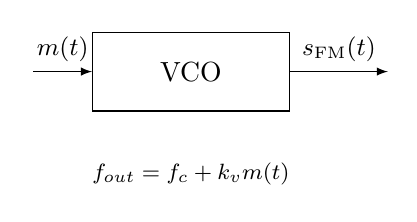
\begin{tikzpicture}[>=latex]
\node[draw, rectangle, minimum width=2.5cm, minimum height=1cm] (vco) at (0,0) {VCO};
\draw[->] (-2,0) -- node[above, font=\small] {$m(t)$} (vco.west);
\draw[->] (vco.east) -- node[above, font=\small] {$s_{\FM}(t)$} (2.5,0);
\node[below of=vco, node distance=1.3cm, font=\footnotesize] {$f_{out} = f_c + k_v m(t)$};
\end{tikzpicture}
\end{center}

\textbf{Características:}
\begin{itemize}
\item Simples e direto
\item $f_{out} = f_c + k_v m(t)$
\item VCO implementado com: varactor diode, capacitor variável, etc.
\end{itemize}

\textbf{Problema:} Instabilidade de frequência

\begin{itemize}
\item $f_c$ pode derivar com temperatura, componentes
\item Difícil obter $f_c$ precisa e estável
\end{itemize}

\textbf{Solução:} Usar método indireto (Armstrong)

\end{frame}

% ============================================

\begin{frame}{Método de Armstrong (Indireto)}

\textbf{Ideia:} Gerar NBFM estável, depois converter para WBFM

\textbf{Processo:}

\begin{enumerate}
\item Gerar NBFM com $\beta$ pequeno e $f_c$ estável (cristal)
\item Multiplicar frequência por $n$:
   \begin{itemize}
   \item $f_c \to nf_c$
   \item $\beta \to n\beta$
   \item $\Delta f \to n\Delta f$
   \end{itemize}
\item Converter para banda desejada (mixing)
\item Repetir multiplicação se necessário
\end{enumerate}

\vspace{0.3cm}

\textbf{Exemplo:}

Gerar FM com $f_c = 100$ MHz, $\Delta f = 75$ kHz:

\begin{itemize}
\item NBFM: $f_1 = 200$ kHz, $\Delta f_1 = 25$ Hz
\item Multiplicar por $\times 64$: $f_2 = 12.8$ MHz, $\Delta f_2 = 1.6$ kHz
\item Multiplicar por $\times 48$: $f_3 = 614.4$ MHz, $\Delta f_3 = 76.8$ kHz
\item Misturar com 514.4 MHz: $f_c = 100$ MHz, $\Delta f = 76.8$ kHz $\approx 75$ kHz
\end{itemize}

\end{frame}

% ============================================

\subsection{Receptor Superheterodino}

\begin{frame}{Princípio do Receptor Superheterodino}

\textbf{Problema:} Demodular diretamente em $f_c$ variável é complexo

\textbf{Solução:} Converter todas as frequências recebidas para uma \textbf{frequência intermediária (IF)} fixa

\begin{center}
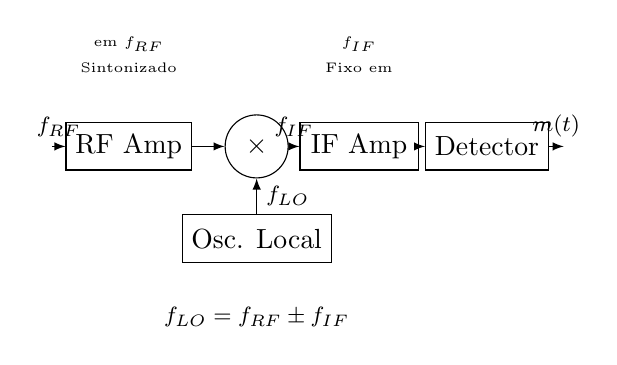
\begin{tikzpicture}[>=latex, scale=0.65]
% Blocos
\node[draw, rectangle, minimum width=1.5cm, minimum height=0.6cm] (rf) at (0,0) {RF Amp};
\node[draw, circle, minimum size=0.8cm] (mix) at (2.5,0) {$\times$};
\node[draw, rectangle, minimum width=1.5cm, minimum height=0.6cm] (if) at (4.5,0) {IF Amp};
\node[draw, rectangle, minimum width=1.5cm, minimum height=0.6cm] (det) at (7,0) {Detector};

% Oscilador local
\node[draw, rectangle, minimum width=1.5cm, minimum height=0.6cm] (lo) at (2.5,-1.8) {Osc. Local};

% Conexões
\draw[->] (-1.5,0) -- node[above, font=\footnotesize] {$f_{RF}$} (rf);
\draw[->] (rf) -- (mix.west);
\draw[->] (mix.east) -- node[above, font=\footnotesize] {$f_{IF}$} (if);
\draw[->] (if) -- (det);
\draw[->] (det) -- node[above, font=\footnotesize] {$m(t)$} (8.5,0);
\draw[->] (lo.north) -- node[right, font=\footnotesize] {$f_{LO}$} (mix.south);

% Labels
\node[above of=rf, node distance=1cm, font=\tiny] {Sintonizado};
\node[above of=rf, node distance=1.3cm, font=\tiny] {em $f_{RF}$};
\node[above of=if, node distance=1cm, font=\tiny] {Fixo em};
\node[above of=if, node distance=1.3cm, font=\tiny] {$f_{IF}$};
\node[below of=lo, node distance=1cm, font=\footnotesize] {$f_{LO} = f_{RF} \pm f_{IF}$};
\end{tikzpicture}
\end{center}

\textbf{Relação:}
\[
f_{IF} = |f_{RF} - f_{LO}|
\]

Ajustando $f_{LO}$, qualquer $f_{RF}$ é convertido para $f_{IF}$ fixo.

\end{frame}

% ============================================

\begin{frame}{Vantagens do Superheterodino}

\textbf{Vantagens:}

\begin{enumerate}
\item \textbf{Seletividade:}
   \begin{itemize}
   \item Filtro IF fixo pode ser muito seletivo
   \item Não precisa ajustar filtro ao trocar estação
   \end{itemize}

\item \textbf{Sensibilidade:}
   \begin{itemize}
   \item Amplificação concentrada em frequência fixa
   \item Melhor controle de ganho (AGC)
   \end{itemize}

\item \textbf{Estabilidade:}
   \begin{itemize}
   \item Osciladores em frequência fixa são mais estáveis
   \end{itemize}
\end{enumerate}

\textbf{Problema: Frequência Imagem}

Duas frequências produzem mesmo $f_{IF}$:
\begin{itemize}
\item Desejada: $f_s = f_{LO} + f_{IF}$
\item Imagem: $f_{im} = f_{LO} - f_{IF}$
\end{itemize}

\textbf{Solução:} Filtro de RF rejeita frequência imagem antes do mixer

\end{frame}

% ============================================

\begin{frame}{Exemplo: Receptor FM Superheterodino}

\textbf{Rádio FM comercial:}

\begin{itemize}
\item Banda FM: 88-108 MHz
\item IF padrão: $f_{IF} = 10.7$ MHz
\end{itemize}

\textbf{Para receber} $f_{RF} = 100.0$ MHz:

\[
f_{LO} = f_{RF} + f_{IF} = 100.0 + 10.7 = 110.7 \text{ MHz}
\]

\textbf{Frequência imagem:}
\[
f_{im} = f_{LO} + f_{IF} = 110.7 + 10.7 = 121.4 \text{ MHz}
\]

Fora da banda FM (88-108 MHz) $\rightarrow$ filtro RF facilmente rejeita

\vspace{0.3cm}

\textbf{Processamento:}
\begin{itemize}
\item Amplificador RF sintonizado em 100 MHz
\item Mixer com LO de 110.7 MHz
\item Amplificador IF em 10.7 MHz (filtro muito seletivo)
\item Discriminador FM ou PLL para demodular
\end{itemize}

\end{frame}

% ============================================

\subsection{FDM}

\begin{frame}{Multiplexação por Divisão de Frequência}

\textbf{FDM (Frequency Division Multiplexing):}

Múltiplos sinais compartilham mesmo canal, cada um em frequência diferente.

\begin{center}
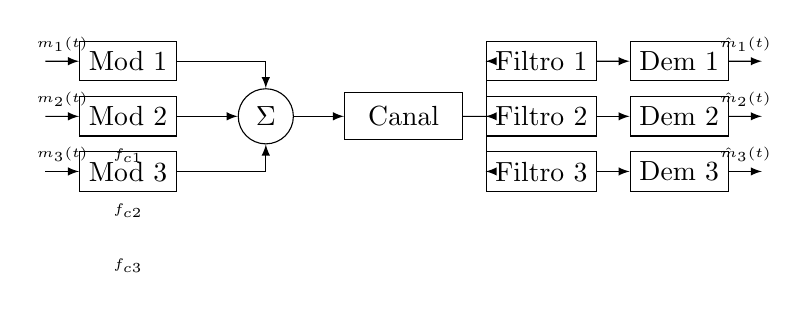
\begin{tikzpicture}[>=latex, scale=0.7]
% Transmissor
\node[draw, rectangle, minimum width=1.2cm, minimum height=0.5cm] (m1) at (0,2) {Mod 1};
\node[draw, rectangle, minimum width=1.2cm, minimum height=0.5cm] (m2) at (0,1) {Mod 2};
\node[draw, rectangle, minimum width=1.2cm, minimum height=0.5cm] (m3) at (0,0) {Mod 3};
\node[draw, circle, minimum size=0.7cm] (sum) at (2.5,1) {$\Sigma$};
\node[draw, rectangle, minimum width=1.5cm, minimum height=0.6cm] (canal) at (5,1) {Canal};

% Receptor
\node[draw, rectangle, minimum width=1.2cm, minimum height=0.5cm] (f1) at (7.5,2) {Filtro 1};
\node[draw, rectangle, minimum width=1.2cm, minimum height=0.5cm] (f2) at (7.5,1) {Filtro 2};
\node[draw, rectangle, minimum width=1.2cm, minimum height=0.5cm] (f3) at (7.5,0) {Filtro 3};
\node[draw, rectangle, minimum width=1.2cm, minimum height=0.5cm] (d1) at (10,2) {Dem 1};
\node[draw, rectangle, minimum width=1.2cm, minimum height=0.5cm] (d2) at (10,1) {Dem 2};
\node[draw, rectangle, minimum width=1.2cm, minimum height=0.5cm] (d3) at (10,0) {Dem 3};

% Conexões TX
\draw[->] (-1.5,2) -- node[above, font=\tiny] {$m_1(t)$} (m1);
\draw[->] (-1.5,1) -- node[above, font=\tiny] {$m_2(t)$} (m2);
\draw[->] (-1.5,0) -- node[above, font=\tiny] {$m_3(t)$} (m3);
\draw[->] (m1) -| (sum.north);
\draw[->] (m2) -- (sum.west);
\draw[->] (m3) -| (sum.south);
\draw[->] (sum) -- (canal);

% Conexões RX
\draw (canal.east) -- (6.5,1);
\draw[->] (6.5,1) |- (f1);
\draw[->] (6.5,1) -- (f2);
\draw[->] (6.5,1) |- (f3);
\draw[->] (f1) -- (d1);
\draw[->] (f2) -- (d2);
\draw[->] (f3) -- (d3);
\draw[->] (d1) -- node[above, font=\tiny] {$\hat{m}_1(t)$} (11.5,2);
\draw[->] (d2) -- node[above, font=\tiny] {$\hat{m}_2(t)$} (11.5,1);
\draw[->] (d3) -- node[above, font=\tiny] {$\hat{m}_3(t)$} (11.5,0);

% Portadoras
\node[below of=m1, node distance=1.2cm, font=\tiny] {$f_{c1}$};
\node[below of=m2, node distance=1.2cm, font=\tiny] {$f_{c2}$};
\node[below of=m3, node distance=1.2cm, font=\tiny] {$f_{c3}$};
\end{tikzpicture}
\end{center}

\textbf{Requisito:} $f_{ci}$ suficientemente espaçadas para evitar sobreposição espectral

\textbf{Aplicações:} TV a cabo, telefonia analógica (hierarquia FDM)

\end{frame}

% ============================================

\begin{frame}{Exemplo: FDM em Telefonia}

\textbf{Hierarquia FDM analógica (histórica):}

\begin{itemize}
\item \textbf{Grupo:} 12 canais de voz (4 kHz cada)
  \begin{itemize}
  \item SSB-LSB, espaçamento de 4 kHz
  \item Faixa: 60-108 kHz
  \item Banda total: 48 kHz
  \end{itemize}

\item \textbf{Supergrupo:} 5 grupos = 60 canais
  \begin{itemize}
  \item Faixa: 312-552 kHz
  \item Banda: 240 kHz
  \end{itemize}

\item \textbf{Grupo mestre:} 10 supergrupos = 600 canais
  \begin{itemize}
  \item Faixa: 564-3084 kHz
  \item Banda: 2520 kHz
  \end{itemize}
\end{itemize}

\vspace{0.3cm}

\textbf{Nota:} Substituído por sistemas digitais (TDM, SONET/SDH), mas princípio permanece em sistemas ópticos (WDM).

\end{frame}

% ============================================

\begin{frame}{Resumo: Modulação Angular}

\textbf{FM vs. PM:}
\begin{itemize}
\item FM: frequência $\propto m(t)$, fase $\propto \int m(t)$
\item PM: fase $\propto m(t)$, frequência $\propto dm(t)/dt$
\item FM mais comum (melhor em ruído)
\end{itemize}

\vspace{0.3cm}

\textbf{Espectro FM:}
\begin{itemize}
\item Infinitas bandas laterais (Bessel)
\item Largura de banda: $B \approx 2(\Delta f + f_m)$ (Carson)
\item NBFM: $\beta \ll 1$, WBFM: $\beta \gg 1$
\end{itemize}

\vspace{0.3cm}

\textbf{Demodulação:}
\begin{itemize}
\item Discriminador de frequência
\item PLL (mais usado atualmente)
\end{itemize}

\vspace{0.3cm}

\textbf{Geração:}
\begin{itemize}
\item Direta: VCO (instável)
\item Indireta: Armstrong (estável)
\end{itemize}

\end{frame}



% %%%%%%%%%%%%%%%%%%%%%%%%%%%%%%%%%%%%%%%%%%%%
% SLIDE DE TRANSIÇÃO: CAPÍTULO 5
% %%%%%%%%%%%%%%%%%%%%%%%%%%%%%%%%%%%%%%%%%%%%
{
\setbeamercolor{background canvas}{bg=structure.fg}
\setbeamercolor{normal text}{fg=white}
\usebeamercolor[fg]{normal text}
\begin{frame}[plain,c]
\begin{center}
{\Huge\textbf{Capítulo 5}}\\[0.8cm]
{\LARGE Efeito do Ruído em Sistemas de Comunicação}\\[0.5cm]
{\large SNR, figura de ruído e perdas de transmissão}
\end{center}
\end{frame}
}

% ============================================
% CAPÍTULO 5: RUÍDO EM SISTEMAS DE COMUNICAÇÃO
% ============================================
\section{Efeito do Ruído em Sistemas de Comunicação}
% ============================================
% EFEITO DO RUÍDO EM SISTEMAS DE COMUNICAÇÃO
% Baseado em Proakis, Cap. 6 - Fundamentals of Communication Systems
% ============================================

\subsection{Ruído em sistema banda base}

\begin{frame}{Modelo de canal com ruído aditivo}

Sistema de comunicação em banda base: sinal $m(t)$ transmitido, ruído aditivo no canal.

\textbf{Sinal recebido:}
\[
r(t) = m(t) + n(t)
\]
onde $n(t)$ é ruído branco gaussiano (AWGN) com densidade espectral de potência bilateral $N_0/2$ (W/Hz).

\vspace{0.3cm}

\textbf{Receptor:} Filtro passa-baixas ideal com largura de banda $W$ (igual à banda de $m(t)$).

\textbf{Potência do sinal na saída do filtro:} $P_m$ (potência média de $m(t)$).

\textbf{Potência do ruído na saída:} Ruído filtrado em $[-W, W]$ tem potência
\[
N = \int_{-W}^{W} \frac{N_0}{2} df = N_0 W
\]

\end{frame}

% ============================================

\begin{frame}{SNR em banda base}

\textbf{Relação sinal-ruído na saída (SNR de referência):}
\[
\left(\frac{S}{N}\right)_o = \frac{P_m}{N_0 W}
\]

\begin{block}{Definição: SNR de entrada}
Chamamos de $\gamma$ a relação sinal-ruído na entrada do demodulador (após filtro de recepção, na banda do sinal):
\[
\gamma = \frac{P_r}{N_0 W}
\]
onde $P_r$ é a potência do sinal recebido (na banda útil).
\end{block}

Para banda base, $P_r = P_m$, logo $(S/N)_o = \gamma$. Este valor serve de \textbf{referência} para comparar modulações.

\end{frame}

% ============================================

\begin{frame}{Exemplo: SNR banda base}

\textbf{Dados:} Sinal de voz com $P_m = 10$ mW, banda $W = 4$ kHz. Canal com $N_0 = 10^{-12}$ W/Hz.

\textbf{Potência do ruído na saída do filtro:}
\[
N = N_0 W = 10^{-12} \times 4000 = 4 \times 10^{-9} \text{ W} = 4 \text{ nW}
\]

\textbf{SNR na saída:}
\[
\left(\frac{S}{N}\right)_o = \frac{10 \times 10^{-3}}{4 \times 10^{-9}} = 2{,}5 \times 10^6 \approx 64 \text{ dB}
\]

\textbf{Parâmetro $\gamma$:}
\[
\gamma = \frac{P_m}{N_0 W} = \left(\frac{S}{N}\right)_o = 64 \text{ dB}
\]

Em sistemas reais, perdas de propagação reduzem $P_r$ e portanto $\gamma$ e $(S/N)_o$.

\end{frame}

% ============================================

\subsection{Ruído em DSB-SC}

\begin{frame}{Receptor DSB-SC com ruído}

Sinal recebido: $r(t) = s(t) + n(t)$, com $s(t) = A_c m(t)\cos(2\pi f_c t)$.

Ruído $n(t)$ em banda passante (centrado em $f_c$): pode ser escrito na forma em quadratura:
\[
n(t) = n_c(t)\cos(2\pi f_c t) - n_s(t)\sin(2\pi f_c t)
\]
onde $n_c(t)$ e $n_s(t)$ são ruídos de banda base, independentes, cada um com PSD $N_0$ em $[-W, W]$ e potência $N_0 W$.

\vspace{0.3cm}

\textbf{Demodulação coerente:} Multiplicar por $2\cos(2\pi f_c t)$ e filtrar passa-baixas em $W$.

Saída do multiplicador:
\[
r(t) \cdot 2\cos(2\pi f_c t) = 2A_c m(t)\cos^2(2\pi f_c t) + 2n(t)\cos(2\pi f_c t)
\]
\[
= A_c m(t)[1+\cos(4\pi f_c t)] + n_c(t)[1+\cos(4\pi f_c t)] + n_s(t)\sin(4\pi f_c t)
\]

Após filtro passa-baixas (remove componentes em $2f_c$):
\[
y(t) = A_c m(t) + n_c(t)
\]

\end{frame}

% ============================================

\begin{frame}{SNR na saída do DSB-SC}

Saída do demodulador: $y(t) = A_c m(t) + n_c(t)$.

\textbf{Potência do sinal na saída:} $P_{so} = A_c^2 P_m$.

\textbf{Potência do ruído na saída:} $n_c(t)$ tem PSD $N_0$ em $[-W,W]$, logo $N_o = N_0 W$.

\textbf{SNR na saída:}
\[
\left(\frac{S}{N}\right)_o = \frac{A_c^2 P_m}{N_0 W}
\]

\textbf{Potência recebida} (sinal DSB-SC): $P_r = \frac{A_c^2 P_m}{2}$ (em 1$\Omega$). Assim $A_c^2 P_m = 2P_r$.

\[
\left(\frac{S}{N}\right)_o = \frac{2P_r}{N_0 W} = 2\gamma
\]

\begin{block}{Resultado}
Para DSB-SC com demodulação coerente: $(S/N)_o = 2\gamma$. Ou seja, \textbf{3 dB melhor} que o sistema banda base de referência (que tem $(S/N)_o = \gamma$ quando $P_r = P_m$). Na prática, a comparação justa é mesma $P_r$: então banda base com $P_r$ tem $(S/N)_o = P_r/(N_0 W) = \gamma$; DSB-SC com mesma $P_r$ tem $(S/N)_o = 2P_r/(N_0 W) = 2\gamma$.
\end{block}

\end{frame}

% ============================================

\begin{frame}{Comparação banda base vs.\ DSB-SC}

\textbf{Banda base:} $(S/N)_o = P_m/(N_0 W)$. Se a potência recebida é $P_m$, então $(S/N)_o = \gamma$.

\textbf{DSB-SC:} Potência transmitida em banda lateral é $P_r = A_c^2 P_m/2$. SNR na saída:
\[
\left(\frac{S}{N}\right)_o = \frac{A_c^2 P_m}{N_0 W} = \frac{2P_r}{N_0 W} = 2\gamma
\]

\textbf{Interpretação:} No DSB-SC, após multiplicação por portadora e filtragem, apenas a componente em fase do ruído ($n_c$) passa; a componente em quadratura ($n_s$) é rejeitada. O sinal útil é recuperado com ganho. O fator 2 em relação a $\gamma$ aparece porque $\gamma$ foi definido como $P_r/(N_0 W)$ e $P_r$ é a potência do sinal modulado (que é metade da potência na saída do demodulador em termos de contribuição útil $A_c^2 P_m = 2P_r$).

\textbf{Em resumo:} Para mesma potência recebida $P_r$, o DSB-SC coerente oferece $(S/N)_o = 2\gamma$, ou seja, o dobro da SNR de um sistema banda base com a mesma potência de sinal na banda $W$.

\end{frame}

% ============================================

\subsection{Ruído em SSB AM}

\begin{frame}{Ruído em SSB AM}

No SSB, o sinal ocupa apenas metade da banda do DSB (largura $W$ em vez de $2W$).

\textbf{Sinal recebido:} $r(t) = s_{\SSB}(t) + n(t)$, com $s_{\SSB}$ em banda $W$ (USB ou LSB).

\textbf{Demodulação coerente:} Mesmo que DSB-SC (multiplicar por portadora em fase e filtrar em $W$).

\textbf{Análise:} O ruído em banda passante na banda do SSB tem as componentes $n_c$ e $n_s$; após demodulação coerente, apenas $n_c$ contribui na saída, com potência $N_0 W$ (a banda do filtro é $W$).

\textbf{Potência do sinal:} $P_r = A_c^2 P_m/4$ (SSB tem metade da potência de um DSB com mesma amplitude de portadora, pois só uma banda lateral). Saída útil: proporcional a $A_c m(t)$, com potência $A_c^2 P_m/4 = P_r$.

\[
\left(\frac{S}{N}\right)_o = \frac{P_r}{N_0 W} = \gamma
\]

\begin{block}{Resultado}
Para SSB com demodulação coerente e mesma potência recebida $P_r$: $(S/N)_o = \gamma$ (igual ao sistema banda base de referência). Mesma performance que banda base, com economia de banda.
\end{block}

\end{frame}

% ============================================

\subsection{Ruído em AM convencional}

\begin{frame}{Receptor AM convencional com ruído}

Sinal AM: $s(t) = A_c[1 + \mu m_n(t)]\cos(2\pi f_c t)$. Receptor usa \textbf{detector de envelope}.

Entrada do detector: $r(t) = s(t) + n(t)$. Escrevendo $n(t) = n_c(t)\cos(2\pi f_c t) - n_s(t)\sin(2\pi f_c t)$:
\[
r(t) = [A_c(1+\mu m_n) + n_c(t)]\cos(2\pi f_c t) - n_s(t)\sin(2\pi f_c t)
\]

\textbf{Envelope} de $r(t)$:
\[
E(t) = \sqrt{[A_c(1+\mu m_n) + n_c]^2 + n_s^2}
\]

Para \textbf{SNR de entrada alta} ($\gamma \gg 1$), o termo dominante é $A_c(1+\mu m_n)$ e o ruído perturba pouco. Aproximação linear mostra que a componente de ruído na saída é essencialmente $n_c(t)$ (em fase com a portadora).

\textbf{Potência da portadora recebida:} $A_c^2/2$. Potência nas bandas laterais: $A_c^2 \mu^2 P_{m_n}/2$. Potência total:
\[
P_r = \frac{A_c^2}{2}\left(1 + \mu^2 P_{m_n}\right)
\]

\end{frame}

% ============================================

\begin{frame}{SNR na saída do AM convencional}

Para AM com detector de envelope e alta SNR, a análise mostra:
\[
\left(\frac{S}{N}\right)_o \approx \frac{\mu^2 P_{m_n}}{1 + \mu^2 P_{m_n}} \, \gamma
\]

Para tom único com $\mu$ (mensagem normalizada): $P_{m_n} = 1/2$,
\[
\left(\frac{S}{N}\right)_o \approx \frac{\mu^2}{2 + \mu^2} \, \gamma
\]

\begin{block}{Eficiência e SNR}
O fator $\frac{\mu^2}{2+\mu^2}$ é exatamente a \textbf{eficiência de potência} $\eta$ do AM. Como $\eta \leq 1/3$ (máximo em $\mu=1$), temos $(S/N)_o \leq \gamma/3$. Ou seja, AM convencional é \textbf{pior} que banda base, DSB-SC e SSB para mesma $\gamma$.
\end{block}

\textbf{Exemplo:} $\mu = 0{,}8$, $\gamma = 1000$ (30 dB). $(S/N)_o \approx \frac{0{,}64}{2{,}64} \times 1000 \approx 242 \approx 24$ dB. Perda de cerca de 6 dB em relação a $\gamma$.

\end{frame}

% ============================================

\subsection{Ruído em modulação angular (FM/PM)}

\begin{frame}{Modelo de ruído em FM}

Sinal FM recebido: $r(t) = A_c \cos[2\pi f_c t + \phi(t)] + n(t)$, com $\phi(t) = 2\pi k_f \int m(\tau)d\tau$.

Ruído em banda passante: $n(t) = n_c(t)\cos(2\pi f_c t) - n_s(t)\sin(2\pi f_c t)$.

\textbf{Representação de $r(t)$ em envelope e fase:}
\[
r(t) = E(t)\cos[2\pi f_c t + \psi(t)]
\]
onde $E(t)$ é o envelope e $\psi(t)$ a fase. Para \textbf{SNR de entrada alta}, $E(t) \approx A_c$ e a perturbação de fase devido ao ruído é
\[
\psi(t) \approx \phi(t) + \frac{n_s(t)}{A_c}
\]
(componente $n_s$ em quadratura modula a fase). O demodulador FM recupera $\frac{1}{2\pi}\frac{d\psi}{dt}$; o ruído na saída está relacionado a $\frac{1}{A_c}\frac{dn_s}{dt}$ (derivada do ruído), cuja PSD aumenta com $f^2$ na banda de mensagem.

\end{frame}

% ============================================

\begin{frame}{SNR na saída do FM (WBFM)}

A análise completa (Proakis, Cap. 6) para FM com tom único $m(t) = A_m \cos(2\pi f_m t)$ e desvio $\Delta f = k_f A_m$ resulta em:
\[
\left(\frac{S}{N}\right)_o = 3\beta^2 \left(\frac{\Delta f}{f_m}\right)^2 \gamma = 3\beta^2 \gamma
\]
(pois $\beta = \Delta f/f_m$).

\begin{block}{Relação SNR em FM}
Para FM com índice de modulação $\beta$ e mesma $\gamma = P_r/(N_0 W)$ (usando $W$ como banda da mensagem):
\[
\boxed{\left(\frac{S}{N}\right)_o = 3\beta^2 \gamma}
\]
\end{block}

\textbf{Observação:} A banda do sinal FM é $B \approx 2(\Delta f + f_m) = 2f_m(\beta+1)$. Para $\beta$ grande, FM troca \textbf{largura de banda} por \textbf{ganho de SNR}: $(S/N)_o$ cresce com $\beta^2$, enquanto a banda cresce aproximadamente com $\beta$. Isso é o trade-off clássico FM: mais banda $\Rightarrow$ mais imunidade a ruído.

\end{frame}

% ============================================

\begin{frame}{Exemplo: SNR em FM}

\textbf{Dados:} FM com $\beta = 5$, $\gamma = 100$ (20 dB). Banda da mensagem $f_m = 15$ kHz.

\[
\left(\frac{S}{N}\right)_o = 3 \times 25 \times 100 = 7500 \approx 38{,}75 \text{ dB}
\]

Ganho sobre banda base: $38{,}75 - 20 = 18{,}75$ dB (melhoria substancial).

\textbf{Preço:} Banda FM $B \approx 2 \times 15 \times (5+1) = 180$ kHz, enquanto banda base seria $2 \times 15 = 30$ kHz. FM usa 6 vezes mais banda e ganha $\approx 3\beta^2 = 75$ em potência de SNR (cerca de 19 dB).

\textbf{Comparação com AM:} Para mesmo $\gamma$, AM convencional daria $(S/N)_o \approx \eta \gamma \leq \gamma/3$; FM com $\beta=5$ dá $75\gamma$, ou seja, FM pode ser muito superior em SNR quando há banda disponível.

\end{frame}

% ============================================

\subsection{Efeito de limiar em FM}

\begin{frame}{Efeito de limiar na demodulação FM}

Para \textbf{SNR de entrada baixa}, a aproximação $E(t) \approx A_c$ e $\psi(t) \approx \phi + n_s/A_c$ deixa de ser válida. O envelope e a fase sofrem distorções não lineares.

\textbf{Comportamento típico:}
\begin{itemize}
\item Acima de um certo \textbf{SNR de entrada} (limiar), $(S/N)_o$ segue a curva $3\beta^2 \gamma$.
\item Abaixo do limiar, $(S/N)_o$ cai rapidamente (degradação súbita).
\end{itemize}

O limiar depende de $\beta$: quanto maior $\beta$, maior tende a ser o SNR de entrada necessário para operar acima do limiar.

\textbf{Causa:} Quando o ruído é forte, o vetor (sinal + ruído) pode “inverter” a fase; o discriminador FM interpreta isso como desvio de frequência espúrio, gerando picos de ruído (clique noise) e degradando $(S/N)_o$.

\end{frame}

% ============================================

\begin{frame}{Curva de limiar (qualitativa)}

\begin{center}
\IfFileExists{figures/cap5/fm_threshold.pdf}{%
\includegraphics[width=\figHalf]{figures/cap5/fm_threshold.pdf}}{%
\fbox{\parbox{0.7\textwidth}{\centering\vspace{2cm}$(S/N)_o$ vs.\ $(S/N)_i$ em FM (limiar). Rode \texttt{14\_fm\_threshold.py}\vspace{2cm}}}}
\end{center}

\textbf{Região linear (acima do limiar):} $(S/N)_o = 3\beta^2 \gamma$. \textbf{Abaixo do limiar:} queda rápida de $(S/N)_o$. Em projetos práticos, escolhe-se $\beta$ e ganho de receptor para manter operação acima do limiar no pior caso de $\gamma$.

\end{frame}

% ============================================

\subsection{Pré-ênfase e pós-ênfase em FM}

\begin{frame}{Motivação: ruído em FM e espectro}

Na saída do demodulador FM, a PSD do ruído é aproximadamente \textbf{quadrática} em frequência: $S_{n_o}(f) \propto f^2$ na banda $[0, W]$. Assim, as \textbf{altas frequências} da mensagem sofrem mais ruído que as baixas.

\textbf{Ideia:} Pré-ênfase no transmissor (amplificar altas frequências antes de modular) e pós-ênfase no receptor (atenuar altas frequências após demodular) de forma que a resposta global seja plana e o ruído seja “achatado” na banda, melhorando o SNR percebido para altas frequências.

\end{frame}

% ============================================

\begin{frame}{Filtros de pré-ênfase e pós-ênfase}

\textbf{Pré-ênfase} (no transmissor): filtro passa-altas suave, por exemplo
\[
H_{pe}(f) = 1 + j\frac{f}{f_0} \quad \Rightarrow \quad |H_{pe}(f)|^2 = 1 + (f/f_0)^2
\]
com $f_0$ da ordem de 2--3 kHz (áudio). Assim, altas frequências são enfatizadas antes da modulação FM.

\textbf{Pós-ênfase} (no receptor): filtro inverso (passa-baixas) para equalizar:
\[
H_{de}(f) = \frac{1}{H_{pe}(f)} = \frac{1}{1 + j f/f_0}
\]
Após demodulação FM, o sinal passa por $H_{de}(f)$; a resposta global para o sinal é plana, e a PSD do ruído (que era $\propto f^2$) é multiplicada por $|H_{de}(f)|^2$, resultando em ruído mais uniforme na banda e melhor SNR médio, especialmente nas altas frequências.

\end{frame}

% ============================================

\begin{frame}{Resposta em frequência típica}

\begin{center}
\IfFileExists{figures/cap5/preemphasis_deemphasis.pdf}{%
\includegraphics[width=\figFull]{figures/cap5/preemphasis_deemphasis.pdf}}{%
\fbox{\parbox{0.7\textwidth}{\centering\vspace{2cm}$|H_{pe}(f)|$ e $|H_{de}(f)|$. Rode \texttt{13\_preemphasis\_deemphasis.py}\vspace{2cm}}}}
\end{center}

Constante de tempo $\tau = 1/(2\pi f_0)$ típica: 75 $\mu$s (FM broadcast), correspondendo a $f_0 \approx 2{,}1$ kHz.

\end{frame}

% ============================================

\subsection{Comparação de sistemas analógicos}

\begin{frame}{Tabela comparativa: SNR e banda}

Para mesma potência recebida $P_r$ e mesma banda de mensagem $W$, definindo $\gamma = P_r/(N_0 W)$:

\begin{center}
\small
\begin{tabular}{|l|c|c|}
\hline
\textbf{Sistema} & \textbf{$(S/N)_o$} & \textbf{Banda do sinal} \\
\hline
Banda base & $\gamma$ & $W$ \\
\hline
DSB-SC (coerente) & $2\gamma$ & $2W$ \\
\hline
SSB (coerente) & $\gamma$ & $W$ \\
\hline
AM convencional (envelope) & $\eta \gamma \leq \gamma/3$ & $2W$ \\
\hline
FM (WBFM, índice $\beta$) & $3\beta^2 \gamma$ & $\approx 2(\Delta f + f_m)$ \\
\hline
\end{tabular}
\end{center}

FM troca banda por SNR; AM convencional tem pior SNR que banda base e DSB-SC. SSB iguala banda base em SNR com metade da banda do DSB.

\end{frame}

% ============================================

\begin{frame}{Gráfico comparativo (placeholder)}

\begin{center}
\IfFileExists{figures/cap5/snr_comparison.pdf}{%
\includegraphics[width=\figHalf]{figures/cap5/snr_comparison.pdf}}{%
\fbox{\parbox{0.7\textwidth}{\centering\vspace{2cm}$(S/N)_o$ vs.\ $\gamma$. Rode \texttt{11\_snr\_comparison.py}\vspace{2cm}}}}
\end{center}

\end{frame}

% ============================================

\subsection{Ruído térmico}

\begin{frame}{Caracterização do ruído térmico}

Ruído térmico em resistores e dispositivos: modelo de \textbf{ruído branco gaussiano} em banda limitada.

\textbf{Densidade espectral de potência (bilateral):}
\[
S_n(f) = \frac{N_0}{2} \quad \text{(W/Hz)}
\]
$N_0 = k T$ em W/Hz, com $k = 1{,}38 \times 10^{-23}$ J/K (Boltzmann) e $T$ a temperatura em Kelvin. Para $T = 290$ K: $N_0 \approx 4 \times 10^{-21}$ W/Hz.

\textbf{Potência de ruído em banda $B$ (positiva):}
\[
N = \frac{N_0}{2} \times 2B = N_0 B
\]
(integrando de $-B$ a $B$ na forma bilateral).

\begin{block}{Ruído térmico}
Fonte térmica à temperatura $T$: PSD bilateral $N_0/2 = kT/2$; potência em banda $B$ = $N_0 B$.
\end{block}

\end{frame}

% ============================================

\begin{frame}{Figura: PSD do ruído térmico}

\begin{center}
\IfFileExists{figures/cap5/thermal_noise_psd.pdf}{%
\includegraphics[width=\figHalf]{figures/cap5/thermal_noise_psd.pdf}}{%
\fbox{\parbox{0.65\textwidth}{\centering\vspace{2cm}PSD $N_0/2$ e potência em banda $W$. Rode \texttt{15\_thermal\_noise\_psd.py}\vspace{2cm}}}}
\end{center}

\end{frame}

% ============================================

\subsection{Figura de ruído e temperatura equivalente}

\begin{frame}{Figura de ruído}

Um amplificador (ou dispositivo) não é ideal: adiciona ruído interno. A \textbf{figura de ruído} $F$ mede a degradação de SNR.

\textbf{Definição (ganho disponível):} Com entrada à temperatura de referência $T_0 = 290$ K,
\[
F = \frac{(S_i/N_i)}{(S_o/N_o)}
\]
onde $S_i/N_i$ é a SNR de entrada e $S_o/N_o$ a SNR de saída (ambas em potência). Para amplificador ideal, $F = 1$. Em dB: $\text{NF} = 10\log_{10} F$.

\textbf{Interpretação:} $F$ é a razão entre a SNR de entrada e a SNR de saída. Quanto maior $F$, pior o bloco para o ruído.

\end{frame}

% ============================================

\begin{frame}{Temperatura equivalente de ruído}

Em vez de $F$, pode-se usar a \textbf{temperatura equivalente de ruído} $T_e$:
\[
F = 1 + \frac{T_e}{T_0} \quad \Leftrightarrow \quad T_e = (F-1)T_0
\]

Interpretação: o ruído interno do dispositivo equivale a colocar na entrada uma fonte térmica à temperatura $T_e$ (além de $T_0$). Ruído total de entrada equivalente: $N_0 B$ com $N_0 = k(T_0 + T_e)$.

\textbf{Exemplo:} $F = 2$ (3 dB) $\Rightarrow$ $T_e = 290$ K. $F = 1{,}1$ $\Rightarrow$ $T_e = 29$ K.

\end{frame}

% ============================================

\begin{frame}{Cascata de estágios (Fórmula de Friis)}

Para estágios em cascata com ganhos disponíveis $G_1, G_2, \ldots$ e figuras de ruído $F_1, F_2, \ldots$, a figura de ruído total é
\[
F_{tot} = F_1 + \frac{F_2 - 1}{G_1} + \frac{F_3 - 1}{G_1 G_2} + \cdots
\]

O primeiro estágio domina se $G_1$ for alto: é importante ter baixo ruído (pequeno $F_1$) no primeiro estágio (ex.: LNA no receptor).

\textbf{Exemplo:} Dois estágios: $F_1 = 2$, $G_1 = 10$; $F_2 = 4$. $F_{tot} = 2 + (4-1)/10 = 2{,}3$. Trocar a ordem (pior estágio primeiro) daria $F_{tot} = 4 + (2-1)/G_2$; se $G_2$ for pequeno, a figura total piora muito.

\end{frame}

% ============================================

\begin{frame}{Figura: cascata e Friis}

\begin{center}
\IfFileExists{figures/cap5/noise_figure_cascade.pdf}{%
\includegraphics[width=\figHalf]{figures/cap5/noise_figure_cascade.pdf}}{%
\fbox{\parbox{0.7\textwidth}{\centering\vspace{2cm}$F_{tot}$ vs.\ $G_1$ (Friis). Rode \texttt{12\_noise\_figure\_cascade.py}\vspace{2cm}}}}
\end{center}

\end{frame}

% ============================================

\subsection{Perdas de transmissão}

\begin{frame}{Atenuação e impacto na SNR}

Enlace com \textbf{perda de transmissão} $L$ (adimensional, $L > 1$): potência recebida $P_r = P_t / L$, onde $P_t$ é a potência transmitida.

\textbf{Ruído:} Assume-se que o ruído é adicionado principalmente no receptor (temperatura de ruído do receptor). Então a potência de ruído na entrada do receptor não depende de $L$; apenas o sinal é atenuado.

\textbf{SNR na entrada do receptor:}
\[
\gamma = \frac{P_r}{N_0 W} = \frac{P_t/L}{N_0 W}
\]
Ou seja, um aumento de $L$ (mais perda) reduz $\gamma$ na mesma proporção. Em dB: perda de 3 dB $\Rightarrow$ $\gamma$ cai 3 dB.

\textbf{Tratamento como “bloco” de ruído:} Um atenuador à temperatura $T_0$ tem figura de ruído $F = L$ e temperatura equivalente $T_e = (L-1)T_0$, útil na cadeia de Friis.

\end{frame}

% ============================================

\subsection{Repetidores}

\begin{frame}{Repetidores em enlaces analógicos}

Para enlaces longos, a atenuação pode ser grande demais. \textbf{Repetidores} são usados para reamplificar o sinal.

\textbf{Repetidor analógico (amplificador):} Amplifica sinal + ruído. O ruído é amplificado junto; cada repetidor adiciona ruído interno (figura de ruído). A SNR degrada a cada estágio. Em cascata de $n$ repetidores iguais, a figura total cresce e a SNR final pode ficar limitada.

\textbf{Repetidor regenerativo} (digital): Detecta e regenera símbolos; o ruído não se acumula da mesma forma (cada regeneração “limpa” o sinal, desde que a taxa de erro seja baixa). Em sistemas digitais, repetidores regenerativos são preferidos para enlaces longos.

\textbf{Resumo:} Em comunicação analógica, repetidores amplificadores degradam progressivamente a SNR; o número de repetidores é limitado pelo SNR mínimo aceitável no destino.

\end{frame}

% ============================================

\begin{frame}{Resumo: Efeito do ruído}

\begin{itemize}
\item \textbf{Banda base:} $(S/N)_o = P_m/(N_0 W) = \gamma$ (referência).
\item \textbf{DSB-SC (coerente):} $(S/N)_o = 2\gamma$.
\item \textbf{SSB (coerente):} $(S/N)_o = \gamma$; mesma SNR que banda base, metade da banda do DSB.
\item \textbf{AM convencional:} $(S/N)_o \approx \eta \gamma \leq \gamma/3$; pior que os demais.
\item \textbf{FM (WBFM):} $(S/N)_o = 3\beta^2 \gamma$; ganho em SNR em troca de banda; efeito de limiar.
\item \textbf{Pré/pós-ênfase:} Melhora SNR em altas frequências em FM.
\item \textbf{Figura de ruído e Friis:} $F_{tot} = F_1 + (F_2-1)/G_1 + \cdots$; primeiro estágio crítico.
\item \textbf{Perdas:} Reduzem $\gamma$; repetidores analógicos degradam SNR ao longo da cascata.
\end{itemize}

\end{frame}


% ============================================
% AGRADECIMENTOS
% ============================================
\begin{frame}{Agradecimentos}
\begin{center}
\Large Obrigado pela atenção!

\vspace{1cm}

\normalsize
\textbf{Contato:}\\
\autorEmail

\vspace{0.5cm}

\textbf{\laboratorioFinal}\\
\universidadeFinal

\vspace{0.5cm}

\textbf{Dúvidas?}
\end{center}
\end{frame}

% ============================================
% REFERÊNCIAS
% ============================================
\begin{frame}[allowframebreaks]{Referências}
\nocite{*}
\bibliographystyle{plain}
\bibliography{references}
\end{frame}

\end{document}
